\documentclass[preprint,12pt]{elsarticle}

\usepackage{amssymb}
\usepackage{amsmath}
\usepackage{lineno}
\usepackage{xcolor}
\usepackage{array}
\usepackage{multirow}
\usepackage{pifont}
\usepackage{adjustbox}
\usepackage{booktabs}
\usepackage{rotating}
\usepackage{colortbl}
\usepackage{tabularx}
\usepackage{makecell}
\usepackage{threeparttable}
\usepackage{graphicx}
\graphicspath{{./Figures/}{Figures/}{./}}

\newcommand{\cmark}{\ding{51}}
\newcommand{\xmark}{\ding{55}}
\newcommand{\pmark}{\textcolor{orange}{$\sim$}}

\newcommand{\rev}[1]{\textcolor{blue}{#1}}
\newcommand{\del}[1]{\textcolor{red}{\sout{#1}}}

\journal{Machine Vision and Applications}

\begin{document}

\begin{frontmatter}

%%%%%%%%%%%%%%%%%%%%%%% Title %%%%%%%%%%%%%%%%%%%%%%%
% The title should clearly identify:
% the practical problem; the image-analysis task; the main modelling approach; the application domain.
% Avoid titles such as "Image Classification Using CNN."
\title{An Explainable Comparative Convolutional Neural Network Framework for Road Surface Damage Classification Using Smartphone Pavement Images}

%%%%%%%%%%%%%%%%%%%%%%% Author Details %%%%%%%%%%%%%%%%%%%%%%%
\author[label1]{Jaskaran Singh}
\affiliation[label1]{organization={Department of Software Engineering, University of Europe for Applied Sciences},
            addressline={Konrad-Zuse-Ring 11},
            city={Potsdam},
            postcode={14469},
            state={Brandenburg},
            country={Germany}}

%%%%%%%%%%%%%%%%%%%%%%% Abstract %%%%%%%%%%%%%%%%%%%%%%%
% The abstract should contain approximately 200-250 words and cover: problem background; gap; aim;
% dataset and classes; models and methodology; evaluation; numerical results; XAI findings;
% practical contribution; main limitation or future direction.
\begin{abstract}
Road surface deterioration such as potholes, cracks, and damaged manhole surrounds is a persistent threat to traffic safety, vehicle integrity, and public maintenance budgets in cities worldwide.
Manual road inspection remains slow, costly, and subjective, while many existing automated studies report only headline accuracy and rarely combine a like-for-like comparison of a purpose-built and a pre-trained network with a transparent explanation of model behaviour.
This study addresses the problem of automatically classifying road surface images into three damage categories, namely potholes, cracks, and manholes, using a comparative and explainable convolutional neural network framework.
A custom convolutional neural network was designed as a baseline and compared against a MobileNetV2 transfer-learning model, with both networks trained on a public dataset of 18{,}674 road images and evaluated on an independent test set.
Model behaviour was further interpreted using Gradient-weighted Class Activation Mapping and SHapley Additive exPlanations, and practical feasibility was assessed through efficiency measurements and a robustness analysis under image blur, noise, and brightness changes.
The custom network reached a test accuracy of 63.93\% with a loss of 0.8302 and outperformed MobileNetV2, which reached 55.26\% accuracy with a loss of 1.0370.
Class-level analysis showed that potholes were recognised most reliably while cracks were by far the hardest class, and the explainability maps confirmed that the model attends to genuine pavement regions for potholes and manholes but disperses its attention for cracks.
The framework therefore offers a reproducible and interpretable baseline for automated road damage screening that can support, but not replace, human infrastructure inspection.
\end{abstract}

%%%%%%%%%%%%%%%%%%%%%%% Graphical Abstract %%%%%%%%%%%%%%%%%%%%%%%
% Provide one publication-quality figure summarizing the problem, dataset, preprocessing, models,
% evaluation, Grad-CAM and SHAP, and the main outcome. Short labels, icons, arrows only.
\begin{graphicalabstract}
%\includegraphics{grabs}
% TODO (student): create grabs.pdf summarising problem, dataset, models, evaluation, XAI, outcome.
\end{graphicalabstract}

%%%%%%%%%%%%%%%%%%%%%%% Research Highlights %%%%%%%%%%%%%%%%%%%%%%%
% Provide five highlights, each no more than ~15 words, covering: the problem; the dataset/setting;
% the models compared; the XAI contribution; the most important outcome.
\begin{highlights}
\item A custom CNN and MobileNetV2 are compared for three-class road damage image classification.
\item The custom CNN reaches 63.93\% test accuracy and outperforms MobileNetV2 at 55.26\%.
\item Cracks are the hardest class while potholes are recognised most reliably.
\item Grad-CAM and SHAP confirm the model attends to genuine pavement damage regions.
\item Efficiency and robustness tests show the lightweight model suits practical screening.
\end{highlights}

%%%%%%%%%%%%%%%%%%%%%%% Keywords %%%%%%%%%%%%%%%%%%%%%%%
% Provide five to seven keywords identifying the domain, CNNs, transfer learning, XAI, and the task.
\begin{keyword}
Road damage detection \sep Convolutional neural networks \sep Transfer learning \sep Explainable artificial intelligence \sep Image classification \sep MobileNetV2
\end{keyword}

\end{frontmatter}

\linenumbers

% ============================================================================
% NOTE: The template's "General instructions" section has been removed because
% Rule 1 of that section explicitly instructs the author to delete it after
% completing the write-up. In accordance with Rule 2, every other template
% instruction is preserved below as commented-out text, with the author's
% content written immediately after each instruction block.
% ============================================================================

\section{Introduction}
% The Introduction should establish the practical problem, explain why CNN-based image analysis is
% appropriate, identify the research gap, and state exactly what the study contributes.

\subsection{Application Background and Practical Importance}
% Explain the real-world problem addressed by the project. Cover: the application domain; people,
% organizations, or systems affected; limitations of current manual or conventional approaches;
% consequences of delayed, inaccurate, or expensive assessment; why automated image analysis may be
% useful. Include recent statistics or domain evidence where appropriate, with references.
% A domain-introduction figure may be included (e.g. undamaged versus damaged infrastructure).

Road networks form the physical backbone of modern transportation and directly influence economic activity, public safety, and daily mobility.
Over time, repeated traffic loading, weathering, temperature cycling, and water ingress cause pavement surfaces to deteriorate into potholes, cracks, and damaged manhole surrounds.
These defects increase the risk of traffic accidents, accelerate vehicle wear, raise fuel consumption, and impose substantial repair costs on both drivers and public authorities.
Transportation agencies, municipal maintenance teams, insurers, and ordinary road users are all affected when damage is detected late or assessed inconsistently.
Conventional inspection still relies heavily on manual surveys carried out by trained personnel, which are expensive, slow, subjective, and difficult to scale across the hundreds of thousands of kilometres of road that many countries maintain \cite{maeda2018road, arya2024global}.
Because inspections are often infrequent, minor defects can grow into severe hazards before they are recorded and repaired.
Automated image-based analysis offers a promising alternative because cameras mounted on smartphones, dashcams, or survey vehicles can capture pavement images cheaply and at large scale \cite{vinodhini2024pothole}.
A reliable automated classifier could therefore help authorities prioritise repairs, reduce inspection costs, and improve overall road safety.

\subsection{Machine Learning and Computer Vision Context}
% Introduce image-based machine learning and explain why CNNs are appropriate. Discuss: automatic
% visual feature extraction; local patterns, shapes, textures, colours, spatial structure;
% advantages of CNNs over manual feature engineering; relevance of deep learning to the application;
% challenges caused by limited labelled data.

Image-based machine learning seeks to map raw pixel data to meaningful labels without relying on manually engineered rules.
Convolutional neural networks are particularly well suited to this task because they automatically learn hierarchical visual features directly from images \cite{nguyen2023survey}.
Early convolutional layers capture low-level patterns such as edges and textures, while deeper layers combine these into higher-level shapes and structures that are discriminative for the target classes.
For road damage, this capability is valuable because potholes, cracks, and manholes differ in characteristic textures, shapes, shadows, and spatial structure that are hard to describe with handcrafted features.
Compared with traditional image-processing pipelines based on thresholding or edge detection, convolutional networks generalise better across varied lighting, weather, and surface conditions \cite{nguyen2023survey}.
However, deep networks typically require large volumes of labelled data to train well, and collecting and annotating road images at scale is laborious.
This challenge of limited labelled data motivates both careful data augmentation and the use of transfer learning, which are central themes of this study.

\subsection{Transfer Learning for the Selected Problem}
% Explain why transfer learning is needed. Discuss: limitations of training a deep CNN from random
% initialization; benefits of pre-trained networks; general visual features learned from large
% datasets; feature extraction and fine-tuning; suitability of the selected transfer-learning
% models. Do not write a full technical explanation of each architecture here.

Transfer learning reuses knowledge captured by a network that has already been trained on a very large general-purpose dataset, most commonly ImageNet.
Training a deep network from random initialisation on a modest domain-specific dataset can lead to slow convergence and overfitting, whereas a pre-trained backbone already encodes general visual features such as edges, corners, and textures \cite{pan2009survey}.
These general features can be reused for a new task by replacing and retraining only the final classification layers, a strategy known as feature extraction, or by additionally unfreezing some backbone layers for fine-tuning.
MobileNetV2 is a widely used lightweight architecture that employs depthwise separable convolutions and inverted residual blocks to achieve strong accuracy at low computational cost, which makes it attractive for mobile and edge deployment \cite{sandler2018mobilenetv2}.
For road inspection, where models may eventually run on smartphones or embedded devices, such efficiency is highly relevant.
This study therefore selects MobileNetV2 as the transfer-learning model and compares it against a custom network trained from scratch.
Detailed architectural descriptions are deferred to the Methodology, as recommended for this type of report.

\subsection{Explainable AI and Trustworthiness}
% Explain why interpretability matters. Discuss: risks of relying only on accuracy; possibility of
% background bias or shortcut learning; importance of confirming that the model uses meaningful image
% regions; role of Grad-CAM; role of SHAP; relevance of explainability to users and decision-makers.
% For safety or infrastructure projects, explain consequences of incorrect or unexplained predictions.

Accuracy alone is an insufficient measure of whether a model can be trusted in a safety-relevant application such as road inspection.
A network may reach a seemingly acceptable accuracy while relying on misleading background cues, a problem often described as shortcut learning.
For infrastructure decisions that influence public spending and safety, it is important to confirm that predictions are driven by genuine damage regions rather than irrelevant context.
Explainable artificial intelligence methods address this need by revealing which parts of an image most influence a prediction \cite{dwivedi2023explainable}.
Gradient-weighted Class Activation Mapping, known as Grad-CAM, produces class-specific heatmaps that highlight the image regions most responsible for a decision \cite{selvaraju2017gradcam}.
SHapley Additive exPlanations, known as SHAP, attribute a contribution value to image regions and can indicate both supporting and opposing evidence for a prediction \cite{lundberg2017unified}.
If incorrect or unexplained predictions are acted upon, authorities may waste resources on phantom defects or, more seriously, overlook genuine hazards, so interpretability is essential for responsible deployment.

\subsection{Research Gap}
% Identify what is missing from previous studies. The gap should be specific and supported by the
% literature review. Do not claim that "no study exists" unless verified carefully.

Although many studies apply convolutional networks to road damage, several methodological gaps remain when they are considered together.
A large number of works report a single model and a single headline accuracy without a controlled comparison between a purpose-built network and a pre-trained alternative on the same data and splits.
Class-imbalance effects are frequently acknowledged but seldom analysed at the level of individual damage types, so it is often unclear which class limits overall performance.
Explainability is still under-used in the road damage literature, and where it appears it is usually limited to a single technique rather than a cross-check between complementary methods such as Grad-CAM and SHAP.
Evaluation under realistic image degradation, such as blur, sensor noise, or changing illumination, is rarely reported even though deployed cameras routinely encounter such conditions.
Finally, computational efficiency is often mentioned only in passing, despite being decisive for on-device deployment.
This study responds to these gaps by combining a controlled model comparison, class-level error analysis, dual explainability, robustness testing, and efficiency measurement within a single reproducible framework.

\subsection{Problem Statement}
% State the exact technical and practical problem. Specify: the type of images; the prediction
% target; the number or nature of classes; the main modelling challenge; the practical purpose.

This study addresses the problem of automatically classifying road surface images into the three categories of pothole, crack, and manhole using a comparative and explainable convolutional neural network framework.
The input data consist of colour photographs of road surfaces captured under varied real-world conditions, and the prediction target is the single most likely damage category for each image.
The main modelling challenge is that the three classes differ in sample count and in visual variability, with cracks in particular appearing in many orientations, widths, and densities that are easily confused with other textures.
The practical purpose of the system is to provide an automated screening tool that can flag and categorise road damage from inexpensive imagery, thereby supporting maintenance prioritisation.
The study specifically investigates whether transfer learning can improve predictive performance over a custom network while maintaining computational efficiency and producing visually meaningful explanations.

\subsection{Aim and Objectives}
% Provide one overall aim, then five to seven measurable objectives.

The aim of this study is to develop and evaluate an explainable convolutional neural network framework for the reliable classification of potholes, cracks, and manholes from road surface images.
To achieve this aim, the following measurable objectives are pursued.
\begin{itemize}
    \item Analyse and preprocess a public road damage image dataset for three-class classification.
    \item Develop a custom convolutional neural network as a baseline classifier.
    \item Implement a MobileNetV2 transfer-learning model for the same task.
    \item Compare the predictive performance of both models using accuracy, loss, and class-level metrics.
    \item Evaluate model efficiency through parameter count, model size, and inference time.
    \item Explain model predictions using Grad-CAM and SHAP and assess their agreement.
    \item Analyse class-level errors, robustness under image degradation, and deployment suitability.
\end{itemize}

\subsection{Research Questions}
% Use the exact statements shared with you for the Research Questions.

\begin{itemize}
    \item RQ1: How effectively can image preprocessing and data augmentation prepare the road damage dataset for reliable three-class CNN classification?
    \item RQ2: Does a custom-designed CNN outperform a MobileNetV2 transfer-learning model for classifying road images into potholes, cracks, and manholes?
    \item RQ3: How does classification performance vary across the three damage classes, and which class is the most difficult to recognise?
    \item RQ4: Do Grad-CAM and SHAP explanations show that the model focuses on meaningful road-damage regions rather than irrelevant background areas?
    \item RQ5: How efficient and robust is the custom CNN in terms of inference time, model size, and performance under image degradation such as blur, noise, and brightness changes?
\end{itemize}

\subsection{Contributions and Novelty}
% Begin with a short paragraph, then provide three to five explicit contributions. Do not describe
% the use of standard CNNs alone as novelty.

This study contributes a compact but complete and reproducible pipeline for explainable road damage classification that integrates model comparison, interpretability, robustness, and efficiency analysis.
Rather than presenting a single accuracy figure, it provides a controlled and transparent evaluation that is intended to be reproducible from the released code and trained model.
The explicit contributions are as follows.
\begin{itemize}
    \item A controlled comparison of a custom convolutional neural network and a MobileNetV2 transfer-learning model trained and evaluated on identical road damage data and splits.
    \item A detailed class-level reliability analysis that identifies cracks as the dominant source of error and explains its likely visual causes.
    \item A dual explainability analysis that cross-checks Grad-CAM and SHAP to confirm whether the model attends to genuine pavement damage.
    \item A combined efficiency and robustness evaluation, including inference time, model size, and performance under blur, noise, and brightness changes, to assess practical deployment.
\end{itemize}
The novelty lies not in proposing a new architecture but in the integrated, honest, and reproducible evaluation of an explainable road damage classifier, including a candid account of where the model and its explanations fall short.

\subsection{Report Organization}
% Provide one short paragraph explaining the remaining sections of the report.

The remainder of this report is organised as follows.
Section~\ref{sec:lit} reviews related work on image-based road damage analysis, convolutional and transfer-learning models, preprocessing, evaluation, and explainability, and presents a comparative literature matrix.
Section~\ref{sec:method} describes the dataset, preprocessing, model architectures, training procedure, evaluation framework, explainability methodology, and robustness analysis.
Section~\ref{sec:results} reports the experimental results organised by research question.
Section~\ref{sec:discussion} interprets these results, compares them with the literature, and discusses limitations and future work.
Section~\ref{sec:conclusion} concludes the report.

\section{Literature Review}
\label{sec:lit}
% The Literature Review should be organized by research themes rather than by individual papers or
% generic headings such as "Technique 1".

\subsection{Image-Based Machine Learning in the Application Domain}
% Review how image analysis has been used in the field. Discuss: conventional image-processing
% approaches; classical machine-learning methods; transition toward deep learning; practical
% advantages and continuing challenges.

Research on automated road condition assessment has evolved rapidly over the past decade.
Early systems relied on classical image processing such as edge detection, thresholding, and texture descriptors to identify pavement defects, which required substantial manual tuning and generalised poorly across surfaces and lighting \cite{kheradmandi2022critical}.
The transition toward deep learning was catalysed by large smartphone-based datasets, most notably the work of Maeda and colleagues, who demonstrated that crowdsourced images could support deep neural network detection of road damage at city scale \cite{maeda2018road}.
Subsequent reviews highlighted both the rapid progress and the persistent difficulty of comparing methods fairly because of differing datasets and evaluation protocols \cite{arya2024global}.
Classical machine-learning classifiers that depend on handcrafted features have largely been superseded by end-to-end convolutional approaches that learn features directly from data.
Nevertheless, challenges remain in handling class imbalance, visual ambiguity between defect types, and the cost of large-scale annotation.
These continuing difficulties motivate the present study's focus on careful evaluation rather than solely on raw accuracy.

\subsection{CNN-Based Methods for the Selected Task}
% Review CNN-based studies addressing the same or closely related problem. Discuss: commonly used
% architectures; dataset sizes and class structures; preprocessing strategies; reported performance;
% strengths and weaknesses; unresolved methodological issues. Compare studies rather than describe
% each paper separately.

A broad family of convolutional approaches has been applied to potholes and cracks, ranging from simple classification networks to detection and segmentation models.
Classification-oriented studies have used architectures such as ResNet-18 for pothole categorisation and reported strong accuracy on curated datasets \cite{naik2023pothole, murty2024detection}.
Other recent works have pursued direct pavement-condition rating and in-vehicle pothole estimation, broadening the practical scope of these systems \cite{qureshi2023deep, ruseruka2024augmenting}.
Detection and segmentation studies have applied Faster R-CNN, Mask R-CNN, and transformer-based segmenters to localise damage at the pixel or region level \cite{li2024road, kulambayev2023realtime, guo2023pavement}.
Several real-time detectors based on improved YOLO variants have also been proposed for road and pavement damage, prioritising inference speed for field use \cite{sami2023improved, xing2023improved, wang2024research}.
Reported performance varies widely because datasets differ in size, class structure, and image quality, which makes direct numerical comparison difficult.
Common strengths across these works include the use of transfer learning and data augmentation, while recurring weaknesses include limited class-level error analysis and little attention to interpretability.
Several studies also note that cracks are particularly challenging because of their thin, elongated, and highly variable appearance \cite{tabernik2023automated, zhu2024lightweight}.
Encoder--decoder and U-Net-based segmentation models have become especially popular for fine-grained crack delineation \cite{dibenedetto2023unet, saberironaghi2024depthcracknet}.
This study is positioned as a classification task with an explicit emphasis on comparing a custom and a pre-trained model and on explaining their behaviour.

\subsection{Transfer Learning Architectures}
% Review relevant pre-trained CNN architectures (e.g. MobileNetV2/V3, ResNet50, DenseNet121,
% EfficientNetB0, InceptionV3, Xception). Explain characteristics, efficiency, depth, parameter size,
% suitability, and prior evidence. Only architectures used in the study need detailed coverage.

A number of pre-trained convolutional architectures are commonly adopted for road damage and related visual tasks.
Deep residual networks such as ResNet introduced skip connections that ease the training of very deep models and remain a popular backbone \cite{he2016deep}.
Recent crack-detection architectures increasingly adopt attention mechanisms and multi-scale feature aggregation to improve accuracy \cite{qi2023gmdnet, wang2024crackms}.
For resource-constrained settings, lightweight architectures use depthwise separable convolutions to dramatically reduce computation while preserving accuracy \cite{liu2024pavement}.
MobileNetV2 extends this idea with inverted residuals and linear bottlenecks, achieving a favourable accuracy-to-cost ratio that is well suited to mobile inspection scenarios \cite{sandler2018mobilenetv2}.
Because this study targets a lightweight and potentially deployable system, MobileNetV2 is selected as the representative transfer-learning model, and the remaining architectures are reviewed only for context.

\subsection{Data Preprocessing and Augmentation}
% Review preprocessing methods (resizing, normalization, cropping, contrast enhancement, denoising,
% augmentation, class balancing, domain-specific transforms). Explain which transformations are
% valid and which may damage class information.

Preprocessing and augmentation strongly influence the performance of convolutional models on modest datasets.
Standard preprocessing includes resizing to a fixed input resolution and normalising pixel intensities to a bounded range, which stabilises training.
Data augmentation artificially expands the effective training set by applying label-preserving transformations such as rotation, zoom, flipping, and brightness changes, which improves generalisation and reduces overfitting \cite{xu2023haar}.
Not all transformations are valid for every domain, and care must be taken that augmentation does not destroy class-defining information.
For road surfaces viewed roughly top-down or forward-facing, moderate rotation, zoom, and horizontal flipping are generally acceptable because a defect remains the same class under these operations.
Extreme transformations, by contrast, could distort the appearance of thin cracks or circular manholes and were therefore avoided.
The augmentation strategy adopted in this study follows these principles and is detailed in the Methodology.

\subsection{Model Evaluation and Reliability}
% Review how previous studies evaluate models (accuracy, precision, recall, specificity, F1,
% ROC-AUC, PR-AUC, confusion matrix, Dice/IoU, mAP, top-k, calibration). Critically identify studies
% that rely only on accuracy.

Sound evaluation requires more than a single accuracy value, particularly when classes are imbalanced.
Widely used metrics include accuracy, precision, recall, and the F1-score, together with the confusion matrix, which exposes the specific pattern of misclassifications \cite{nguyen2023survey}.
Macro-averaged metrics treat all classes equally and are therefore more informative than accuracy when minority classes matter.
A recurring criticism of the road damage literature is that many studies rely predominantly on overall accuracy and report little class-level detail, which can mask poor performance on difficult classes.
This study deliberately reports class-wise precision, recall, and F1-score alongside the confusion matrix to provide a more faithful picture of reliability.
It also reports efficiency metrics, which are frequently omitted despite their importance for deployment.

\subsection{Explainable AI in Image Analysis}
% Review XAI methods used in the domain.

\subsubsection{Grad-CAM}
% Discuss how Grad-CAM produces class-specific activation maps; how it has been used; its value for
% inspecting model attention; its limitations including coarse spatial resolution.

Grad-CAM produces class-specific activation maps by weighting the feature maps of a convolutional layer according to the gradient of the target class \cite{selvaraju2017gradcam}.
The resulting heatmap highlights the image regions that most strongly support a given prediction and can be overlaid on the original image for visual inspection.
It has been applied across many domains, including medical imaging and fault diagnosis, to verify that models attend to meaningful regions \cite{li2023multilayer, dhar2023challenges}.
Its main limitation is coarse spatial resolution, because the heatmap inherits the low resolution of the final convolutional layer.
Despite this, it remains one of the most widely used and intuitive explanation techniques.

\subsubsection{SHAP}
% Discuss feature or region contribution; positive and negative support; image masking or
% superpixels; computational cost; interpretation limitations.

SHAP assigns each input region a contribution value derived from cooperative game theory, indicating how much that region pushes the prediction toward or away from a class \cite{lundberg2017unified}.
For images, region-based or masking-based variants estimate these contributions by perturbing parts of the image and observing the change in output.
A key advantage of SHAP is that it can show both positive and negative evidence, offering a more nuanced view than a single activation map.
Recent applied studies combine SHAP, LIME, and Grad-CAM to interpret deep classifiers and to build trust in safety-relevant predictions \cite{nazim2025advancing, deshpande2024explainable, mandloi2024explainable}.
Its main drawback is computational cost, because many model evaluations are required to estimate contributions, and the resulting maps can be sensitive to the choice of background and masking strategy.
In this study SHAP is used to complement Grad-CAM rather than to replace it.

\subsubsection{Explainability Limitations}
% Explain that attractive heatmaps are not proof of correct reasoning. Discuss sensitivity to
% preprocessing; instability; model dependence; possible highlighting of irrelevant regions; need
% for domain-based interpretation.

It is important to stress that an attractive heatmap is not proof of correct reasoning.
Explanation methods can be sensitive to preprocessing, can be unstable across similar inputs, and depend on the underlying model.
A map may highlight an irrelevant region simply because that region happens to influence the output, which does not guarantee a causally correct decision.
Consequently, explanations must be interpreted in the context of domain knowledge and treated as supporting evidence rather than as definitive justification.
This study adopts that cautious stance and reports cases where the explanations are weak or ambiguous.

\subsection{Robustness, Generalization, and Deployment}
% Review studies addressing image noise, blur, illumination, occlusion, domain shift, external
% datasets, mobile/edge deployment, model size, inference time, memory. May be shortened if
% robustness is out of scope, but computational feasibility should still be reviewed.

Deployed inspection cameras routinely encounter blur from motion, sensor noise in low light, and large brightness variations across the day.
A model intended for real use should therefore be evaluated not only on clean images but also under such degradations.
Relatively few road damage studies report this kind of robustness analysis, even when they claim real-world applicability.
Deployment also depends on computational feasibility, including model size, memory use, and inference time, which determine whether a model can run on a smartphone or embedded device \cite{sandler2018mobilenetv2}.
This study includes both a robustness analysis under controlled degradations and an efficiency analysis, so that practical feasibility is assessed alongside accuracy.

\subsection{Comparative Literature Review Matrix}
% Prepare a comparative literature review matrix of ~12-20 closely related peer-reviewed studies with
% the specified columns and tick/cross/partial symbols. The final row must be the proposed study.
% Refer to the table in the main text and synthesize common strengths, recurring weaknesses,
% disagreements, and missing evaluations rather than repeating the table.

Table~\ref{tab:literature_matrix} compares closely related road damage and image-classification studies across datasets, models, evaluation practices, explainability, robustness, validation, and efficiency, and contrasts them with the proposed work.
The comparison shows that transfer learning and multiple-model comparison are common, but that explainability, robustness testing, statistical testing, and efficiency analysis are applied only sporadically.
In particular, very few studies combine Grad-CAM and SHAP, and fewer still pair this with robustness and efficiency measurement on the same model.
The proposed study is therefore positioned to fill this combined gap by reporting a controlled comparison together with dual explainability, robustness, and efficiency analysis.
The matrix entries summarise each study concisely so that the table remains readable, and the symbols indicate whether a given capability is present, absent, or only partially addressed.

\begin{sidewaystable}[p]
\centering
\tiny
\caption{Comparative literature review matrix summarising datasets, models, evaluation practices, explainability, robustness, validation, and efficiency analysis in closely related road damage and image-classification studies, with the proposed study shown in the final row. Symbols: \cmark{} included, \xmark{} not included, \pmark{} partially or weakly addressed. TL: Transfer Learning; CB: Class Balancing; MC: Multiple-Model Comparison; GC: Grad-CAM; SH: SHAP; RT: Robustness Testing; EV: External Validation; ST: Statistical Testing; EA: Efficiency Analysis.}
\label{tab:literature_matrix}
\begin{tabular}{p{1.3cm} p{1.5cm} p{1.2cm} c p{1.0cm} p{1.5cm} p{1.4cm} c c c c c c c c c p{1.4cm} p{2.0cm} p{2.0cm}}
\toprule
\textbf{Study} & \textbf{Problem} & \textbf{Dataset} & \textbf{Cls} & \textbf{Size} & \textbf{Preproc.} & \textbf{Models} & \textbf{TL} & \textbf{CB} & \textbf{MC} & \textbf{GC} & \textbf{SH} & \textbf{RT} & \textbf{EV} & \textbf{ST} & \textbf{EA} & \textbf{Metrics} & \textbf{Main Contribution} & \textbf{Principal Limitation} \\
\midrule
Maeda et al.~\cite{maeda2018road}, 2018 & Road damage detection & Smartphone road damage & 8 & 9{,}053 images & Resize, label boxes & CNN (SSD) & \cmark & \xmark & \pmark & \xmark & \xmark & \xmark & \pmark & \xmark & \pmark & mAP, F1 & Large smartphone dataset and on-device detection & No explainability or robustness analysis \\
Kheradmandi \& Mehranfar~\cite{kheradmandi2022critical}, 2022 & Pavement crack segmentation review & Multiple crack sets & 2 & Survey & Varied (review) & Segmentation CNNs & \cmark & \xmark & \cmark & \xmark & \xmark & \pmark & \xmark & \xmark & \pmark & IoU, F1 & Comparative review of crack segmentation & Review only, no new model \\
Naik \& Dondeti~\cite{naik2023pothole}, 2023 & Pothole classification & Pothole image set & 2 & Several thousand & Resize, augment & ResNet-18 & \cmark & \xmark & \xmark & \xmark & \xmark & \xmark & \xmark & \xmark & \xmark & Accuracy & Transfer learning for pothole classification & Single model and no explainability \\
Murty et al.~\cite{murty2024detection}, 2024 & Pothole detection \& classification & Public pothole data & 2 & Several thousand & Resize, normalize & CNN & \pmark & \xmark & \xmark & \xmark & \xmark & \xmark & \xmark & \xmark & \xmark & Accuracy, F1 & Simple CNN pipeline for potholes & Limited evaluation depth \\
Kortmann et al.~\cite{kortmann2020detecting}, 2020 & Multi-type road damage & RDD global & 4+ & 26{,}000+ images & Resize, augment & Faster R-CNN & \cmark & \pmark & \xmark & \xmark & \xmark & \xmark & \cmark & \xmark & \xmark & mAP & Cross-country damage detection & Heavy detector, no explainability \\
Kulambayev et al.~\cite{kulambayev2023realtime}, 2023 & Road surface damage & Custom set & 4 & Several thousand & Resize, mask label & Mask R-CNN & \cmark & \xmark & \xmark & \xmark & \xmark & \xmark & \xmark & \xmark & \pmark & mAP, IoU & Real-time segmentation framework & No interpretability or robustness \\
Vinodhini \& Sidhaarth~\cite{vinodhini2024pothole}, 2024 & Pothole detection & Bituminous road images & 2 & Several thousand & Resize, augment & CNN + TL & \cmark & \xmark & \pmark & \xmark & \xmark & \xmark & \xmark & \xmark & \xmark & Accuracy & TL improves pothole detection & Binary scope, no XAI \\
Guo et al.~\cite{guo2023pavement}, 2023 & Pavement crack detection & Crack benchmark & 2 & Several thousand & Patch, normalize & Transformer & \cmark & \xmark & \xmark & \xmark & \xmark & \pmark & \xmark & \xmark & \pmark & F1, IoU & Transformer for cracks & No SHAP or efficiency focus \\
Zhu et al.~\cite{zhu2024lightweight}, 2024 & Pavement crack detection & Crack dataset & 2 & Several thousand & Resize, augment & Light encoder--decoder & \cmark & \xmark & \xmark & \xmark & \xmark & \xmark & \xmark & \xmark & \cmark & F1, IoU & Lightweight crack network & Crack-only, no XAI \\
Tabernik et al.~\cite{tabernik2023automated}, 2023 & Concrete crack detection & Concrete surfaces & 2 & Several thousand & Crop, normalize & Seg.\ + Cls.\ CNN & \cmark & \xmark & \pmark & \xmark & \xmark & \xmark & \xmark & \xmark & \xmark & F1, IoU & Joint segmentation \& classification & No interpretability \\
Zhang et al.~\cite{zhang2022road}, 2022 & Road damage (UAV) & UAV road images & 4 & Several thousand & Resize, augment & Attention CNN & \cmark & \pmark & \pmark & \xmark & \xmark & \xmark & \pmark & \xmark & \xmark & mAP & Multi-level attention for UAV images & No XAI, limited robustness \\
Saha et al.~\cite{saha2024federated}, 2024 & Global road damage & RDD multi-country & 4+ & 26{,}000+ images & Resize, augment & Federated CNN & \cmark & \pmark & \cmark & \xmark & \xmark & \xmark & \cmark & \pmark & \pmark & mAP, F1 & Federated global detection & No explainability \\
\textbf{Proposed study} & \textbf{Road damage classification} & \textbf{Public road damage} & \textbf{3} & \textbf{18{,}674 images} & \textbf{Resize 128, norm, augment} & \textbf{Custom CNN, MobileNetV2} & \cmark & \pmark & \cmark & \cmark & \cmark & \cmark & \xmark & \pmark & \cmark & \textbf{Acc, P, R, F1} & \textbf{Explainable, robust, efficient model comparison} & \textbf{Single dataset, one split} \\
\bottomrule
\end{tabular}
\end{sidewaystable}

\subsection{Synthesis of Literature and Identified Gap}
% Do not merely repeat the gap from the Introduction. Synthesize what the literature does well, the
% most common methods, where findings disagree, what is methodologically missing, and how the
% proposed study responds. End with a transition to the Methodology.

Taken together, the reviewed studies consistently demonstrate that convolutional networks outperform handcrafted approaches and that transfer learning and augmentation are now standard practice.
The most common methods are detection and segmentation models trained on smartphone or vehicle imagery, evaluated mainly with accuracy or mean average precision.
Where studies disagree is in reported performance, which varies sharply because datasets, class structures, and evaluation protocols differ, making direct numerical comparison unreliable.
What is methodologically missing across the literature is the consistent combination of class-level error analysis, dual explainability, robustness testing, and efficiency measurement within one controlled study.
Explainability in particular is rare in the road damage domain, and the pairing of Grad-CAM with SHAP is almost absent.
The proposed study responds to these limitations by holding the dataset and splits fixed while comparing a custom and a pre-trained model, and by reporting interpretability, robustness, and efficiency together.
This integrated and honest evaluation, rather than a new architecture, is the contribution that distinguishes the present work and leads directly into the methodology described next.

\section{Methodology}
\label{sec:method}
% The Methodology must describe the complete experimental design in enough detail for another
% researcher to reproduce the study.

\subsection{Research Design}
% State whether the work is experimental and quantitative; the image task type; the comparative
% nature; models evaluated; XAI methods; evaluation strategy. Include an overall workflow figure.

This study follows an experimental and quantitative research design centred on supervised image classification.
The task is single-label classification of road surface images into three mutually exclusive categories, namely pothole, crack, and manhole.
The work is explicitly comparative, evaluating a custom convolutional neural network against a MobileNetV2 transfer-learning model under identical data and training conditions.
Two explainability methods, Grad-CAM and SHAP, are applied to interpret model behaviour, and a robustness analysis together with efficiency measurement assesses practical feasibility.
The overall workflow proceeds from problem and dataset selection, through dataset inspection, cleaning, preprocessing, splitting, and augmentation, to custom CNN development, transfer learning, training and validation, evaluation, explainability, model comparison, and finally practical interpretation.
Figure~\ref{Fig:Workflow} presents this workflow as a single diagram.

\begin{figure*}[!ht]
\centerline{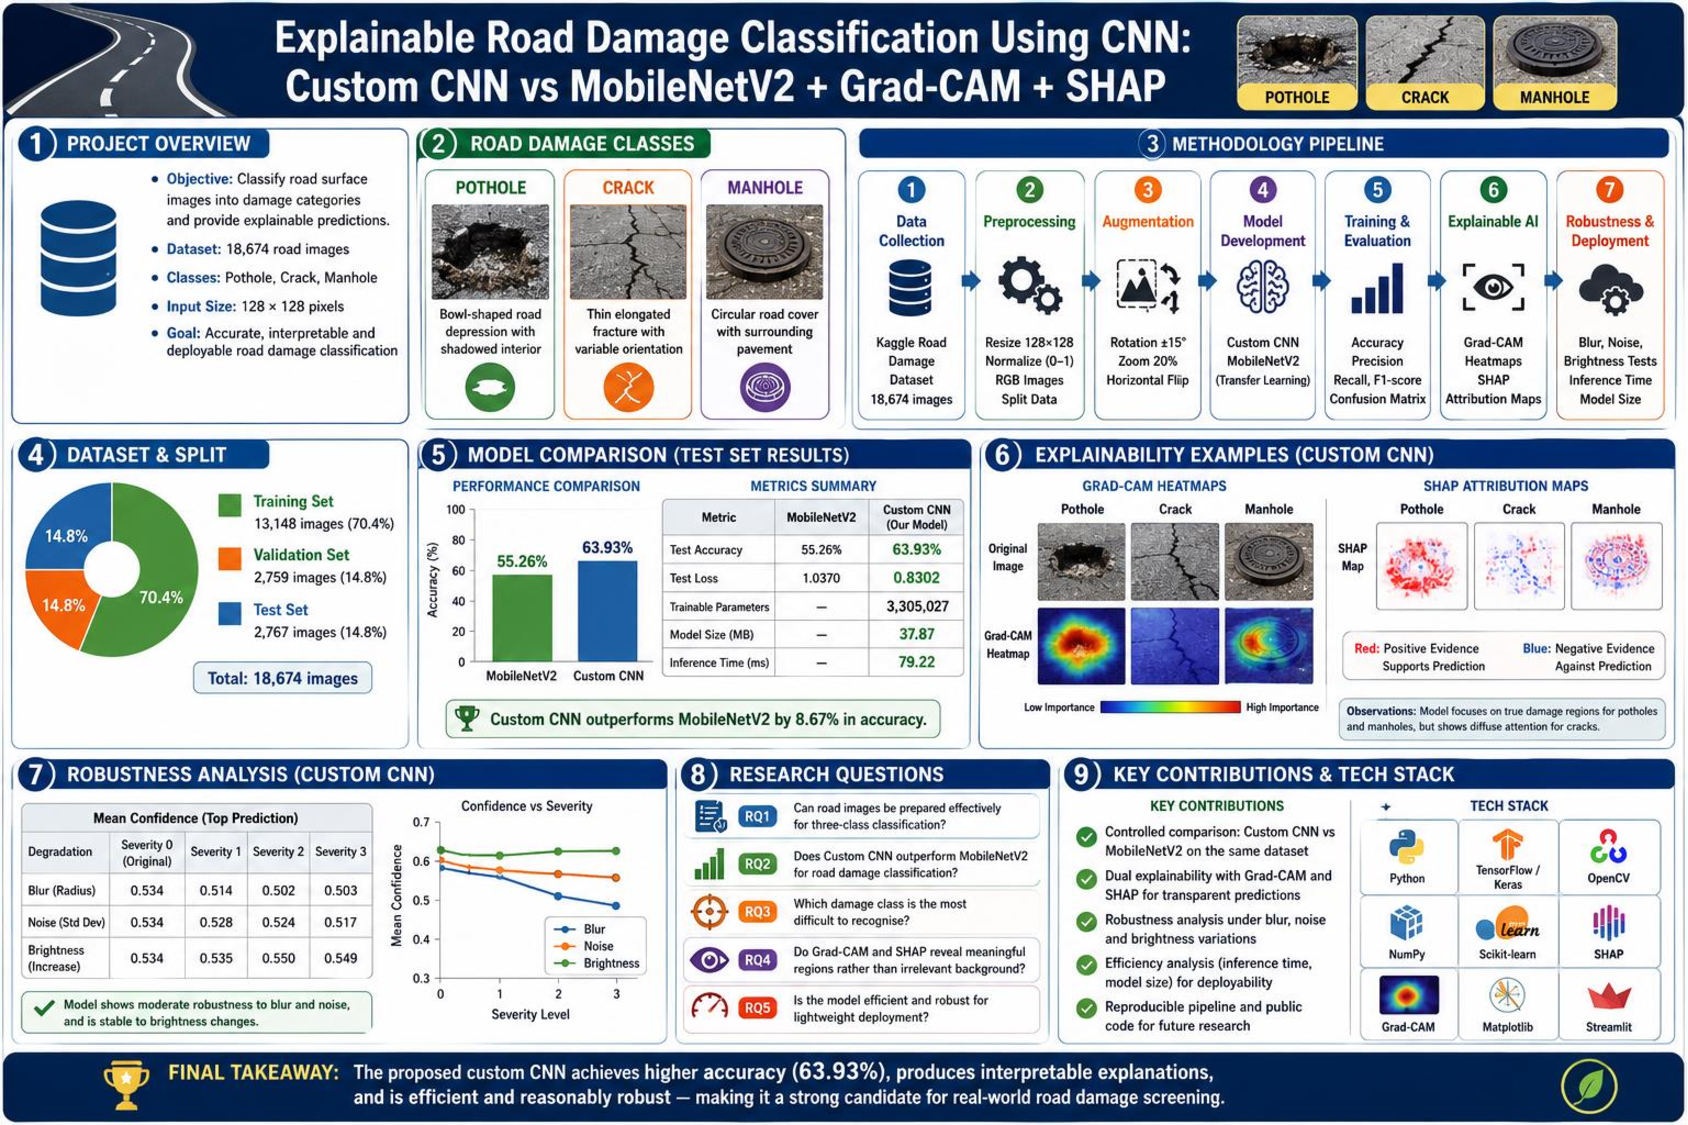
\includegraphics[width=15cm]{./Figures/workflow.pdf}}
\caption{Overall workflow of the proposed explainable road damage classification framework, showing the progression from dataset selection and preprocessing, through custom CNN and MobileNetV2 development, model training and evaluation, to Grad-CAM and SHAP explainability, robustness testing, and efficiency analysis. Each numbered stage corresponds to a methodological step described in this section.}
\label{Fig:Workflow}
\end{figure*}
% TODO (student): create workflow.pdf in PowerPoint/Canva following the template's figure guidelines
% (numbered coloured circles, sub-steps in rectangles, coloured arrows, icons with 2-3 word labels,
% white background). Save as PDF into the Figures folder.

\subsection{Dataset Description}

\subsubsection{Dataset Source and Accessibility}
% State dataset name; creator or repository; URL; access date; license; reason for selection.

The dataset used in this study is the publicly available Road Damage Dataset hosted on Kaggle.
It was selected because it provides a large number of real-world road surface images organised into the damage categories relevant to this project, and because its public availability supports reproducibility.
The dataset is accessible at the Kaggle repository \texttt{anderfian/road-damage-dataset} and was accessed during the project period in 2026.
The images were captured under varied real-world conditions, which makes the dataset suitable for evaluating a practical classification model.
Use of a public dataset also means that no new data collection from human subjects was required.

\subsubsection{Dataset Composition}
% Report total images; classes; images per class; formats; resolutions; existing train/test folders;
% annotation type; missing, corrupt, or duplicate samples.

The dataset comprises 18{,}674 road surface images distributed across three classes.
It is divided into a training set of 13{,}148 images, a validation set of 2{,}759 images, and an independent test set of 2{,}767 images, corresponding to approximately 70\%, 15\%, and 15\% of the data respectively.
The images are stored in JPEG format and were resized to a common resolution of $128 \times 128$ pixels for model input.
The three classes are pothole, crack, and manhole, encoded as integer labels zero, one, and two respectively.
Table~\ref{tab:dataset} summarises the split composition and Table~\ref{tab:classes} summarises the class definitions.

\begin{table}[!ht]
\centering
\caption{Composition of the road damage dataset showing the number of images and the approximate percentage of the total in the training, validation, and independent test splits used throughout this study.}
\label{tab:dataset}
\begin{tabular}{lrr}
\toprule
\textbf{Split} & \textbf{Images} & \textbf{Percentage} \\
\midrule
Training   & 13{,}148 & 70.4\% \\
Validation & 2{,}759  & 14.8\% \\
Testing    & 2{,}767  & 14.8\% \\
\midrule
\textbf{Total} & \textbf{18{,}674} & \textbf{100\%} \\
\bottomrule
\end{tabular}
\end{table}

\begin{table}[!ht]
\centering
\caption{Definitions of the three road damage classes used in this study, including the integer label used during training and the principal visual characteristics that distinguish each class from the others.}
\label{tab:classes}
\begin{tabular}{cll}
\toprule
\textbf{Label} & \textbf{Class} & \textbf{Visual characteristics} \\
\midrule
0 & Pothole & Bowl-shaped depression with shadowed interior \\
1 & Crack   & Thin elongated fracture, variable orientation \\
2 & Manhole & Circular cover and surrounding pavement \\
\bottomrule
\end{tabular}
\end{table}

\subsubsection{Class Definitions}
% Define each class clearly and explain what distinguishes it from the others.

Each class is defined by characteristic visual properties that distinguish it from the others.
A pothole is a bowl-shaped depression in the road surface, typically displaying a darker shadowed interior and an irregular broken edge.
A crack is a thin and elongated surface fracture that can appear in many orientations, widths, and branching patterns, and is often low in contrast against the surrounding pavement.
A manhole is a circular metal or concrete cover set into the road, usually surrounded by intact pavement and sometimes by minor radial cracking.
The principal source of ambiguity is that cracks are thin and visually subtle, so they can resemble ordinary surface texture or the broken edge of a pothole.

\subsubsection{Dataset Quality Assessment}
% Discuss class imbalance; duplicates; low-resolution samples; irrelevant backgrounds; label noise;
% possible data leakage; source or acquisition bias.

Several data quality factors were considered before training.
The three classes are not perfectly balanced, with the crack class being comparatively under-represented in the effective test distribution, which has a direct impact on class-level performance.
Some images contain substantial background such as roadside vegetation, sky, or buildings, which introduces irrelevant context that the model must learn to ignore.
A small number of images include watermarks or text overlays typical of stock photography, which are a potential source of spurious cues.
Because the dataset is supplied with predefined splits, the risk of obvious data leakage between training and testing is reduced, although the absence of an external dataset means generalisation beyond this source remains untested.
These observations motivate both the augmentation strategy and the explainability analysis, which together help reveal whether the model relies on genuine damage features.

\subsubsection{Dataset Visualization}
% Include representative images from every class; class-distribution plot; image-size distribution if
% relevant; examples of challenging images.

Representative images from each class, together with a class-distribution plot, are provided in Figure~\ref{Fig:Dataset} to illustrate the visual variety and the relative class frequencies.
The visualisation highlights the comparatively small number of crack images and the visual subtlety of that class.

\begin{figure}[!ht]
\centerline{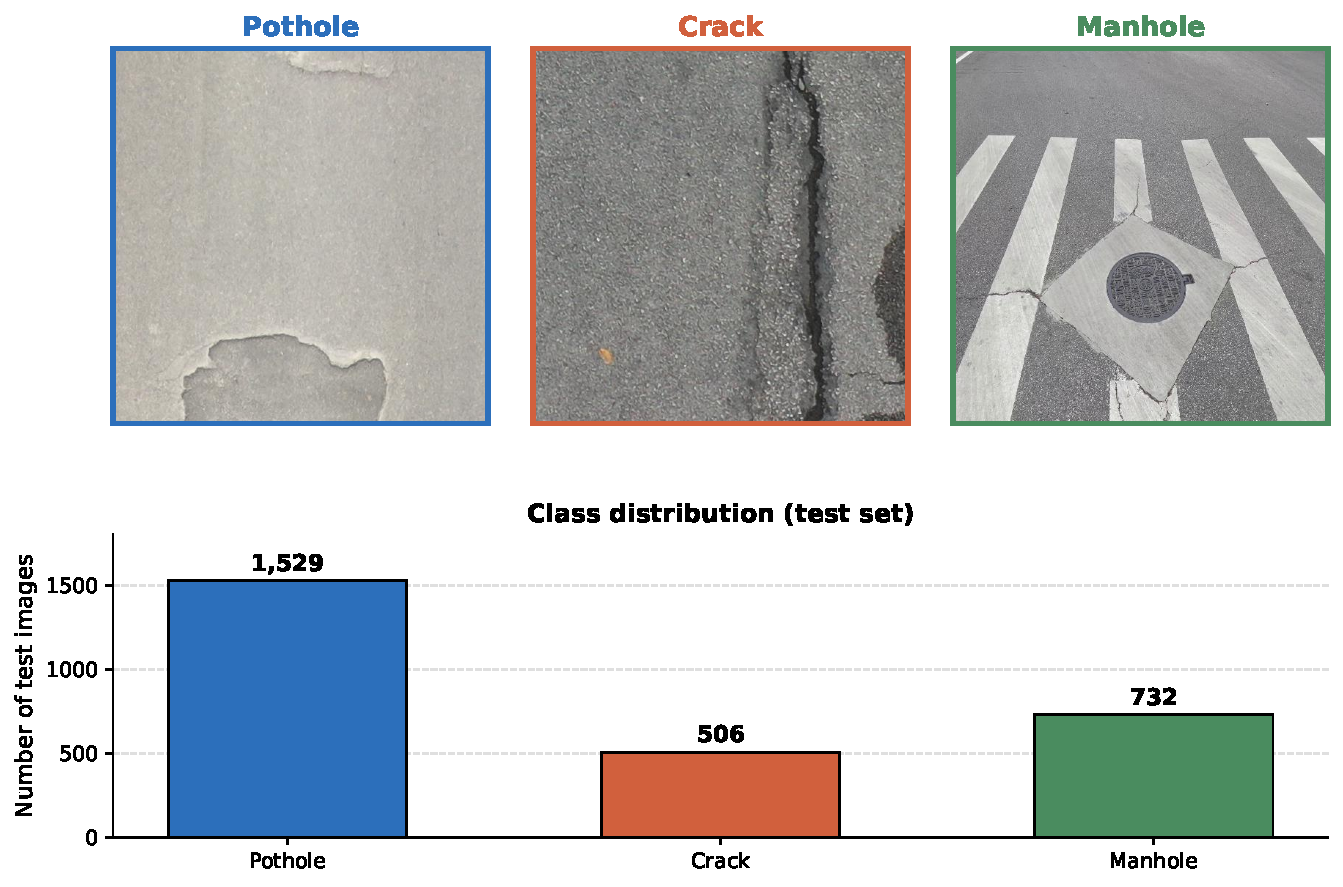
\includegraphics[width=8.9cm]{./Figures/dataset_samples.pdf}}
\caption{Representative sample images from each of the three road damage classes together with the class-distribution of the dataset, illustrating both the visual variability within each class and the relative frequency of potholes, cracks, and manholes.}
\label{Fig:Dataset}
\end{figure}
% TODO (student): create dataset_samples.pdf showing a few images per class plus a class-count bar chart.

\subsection{Data Preparation}

\subsubsection{Data Cleaning}
% Explain corrupt-image removal; duplicate detection; label verification; exclusion criteria;
% handling of unreadable files.

Before training, the dataset was checked for unreadable or corrupt image files, which were excluded from further processing.
Because the dataset is curated and supplied with a defined class structure, extensive relabelling was not required.
Images that could not be opened or decoded were skipped during loading so that they did not interrupt training.
No aggressive deduplication was performed, as the predefined splits already separate the data into training, validation, and test partitions.
The cleaning stage therefore focused on ensuring that every image used was readable and correctly associated with its class label.

\subsubsection{Data Splitting}
% State exact proportions or counts for train/val/test. Use stratified splitting where appropriate.
% Prevent data leakage across splits.

The dataset was used with its predefined partition into training, validation, and independent test sets, as reported in Table~\ref{tab:dataset}.
The training set was used to fit model parameters, the validation set to monitor generalisation during training, and the test set was held out entirely until final evaluation.
Keeping the test set untouched during training prevents optimistic bias in the reported results.
Because the splits are provided with the dataset, the same partition was applied identically to both the custom CNN and the MobileNetV2 model, which is essential for a fair comparison.
This consistent splitting ensures that any observed performance difference reflects the models rather than differences in data.

\subsubsection{Image Preprocessing}
% Explain target image size; colour mode; pixel normalization; resizing method; cropping; contrast
% enhancement; domain-specific preprocessing. Justify each operation.

All images were converted to three-channel colour and resized to a fixed resolution of $128 \times 128$ pixels, which balances visual detail against computational cost.
Pixel intensities were normalised from the original zero-to-255 range into the zero-to-one range by dividing by 255, which stabilises optimisation.
A fixed input size is required so that batches of images can be processed efficiently by the network.
The $128 \times 128$ resolution was chosen as a practical compromise that preserves enough detail for potholes and manholes while keeping the model small, although it inevitably reduces the visibility of very thin cracks.
The same preprocessing was applied identically across training, validation, and test images, except that augmentation was restricted to training.

\subsubsection{Data Augmentation}
% List applied transformations and parameter ranges. Explain why each is valid for the application.

To improve generalisation and reduce overfitting, online data augmentation was applied to the training images only.
The augmentation pipeline applied random rotation of up to 15 degrees, random zoom of up to 20\%, and random horizontal flipping.
Rotation reflects the fact that road damage can appear at slightly different orientations depending on camera angle.
Zoom simulates variation in the distance between the camera and the road surface.
Horizontal flipping is valid because a defect retains its class when mirrored left to right.
These transformations were deliberately kept moderate so that they would not distort the defining appearance of thin cracks or circular manholes.
Validation and test images were never augmented, so that evaluation reflects performance on unmodified data.

\subsubsection{Class-Imbalance Handling}
% Explain whether class weights, oversampling, targeted augmentation, undersampling, focal loss, or
% no balancing was used, and the reason.

The dataset exhibits moderate class imbalance, with cracks under-represented relative to potholes.
In this study, imbalance was addressed indirectly through data augmentation rather than through explicit class weighting or oversampling.
This choice keeps the training pipeline simple and reproducible, which is appropriate for a baseline comparative study.
However, the absence of explicit balancing is acknowledged as a limitation, because it contributes to the poor recall observed for the crack class.
Future work could introduce class weights or targeted oversampling to mitigate this effect.

\subsection{Model Development}

\subsubsection{Custom CNN Baseline}
% Describe input dimensions; conv layers; filter sizes; activations; pooling; batch norm; dropout;
% FC layers; output layer; loss. Include an architecture figure or table.

The custom convolutional neural network was designed specifically for three-class road damage classification.
It accepts an input of size $128 \times 128 \times 3$ and consists of three convolutional blocks followed by a classification head.
Each convolutional block contains a two-dimensional convolution with a $3 \times 3$ kernel and rectified linear unit activation, followed by $2 \times 2$ max pooling for spatial downsampling.
The three blocks use 32, 64, and 128 filters respectively, allowing the network to extract progressively higher-level features.
After the final pooling operation, the feature maps are flattened and passed to a dense layer of 128 units with rectified linear unit activation, followed by a dropout layer with a rate of 0.5 for regularisation, and finally a dense output layer of three units with softmax activation.
The model was compiled with the Adam optimiser and a cross-entropy loss appropriate to multi-class classification.
The complete architecture is summarised in Figure~\ref{Fig:Architecture}, and the network contains approximately 3.31 million trainable parameters.

\begin{figure*}[!ht]
\centerline{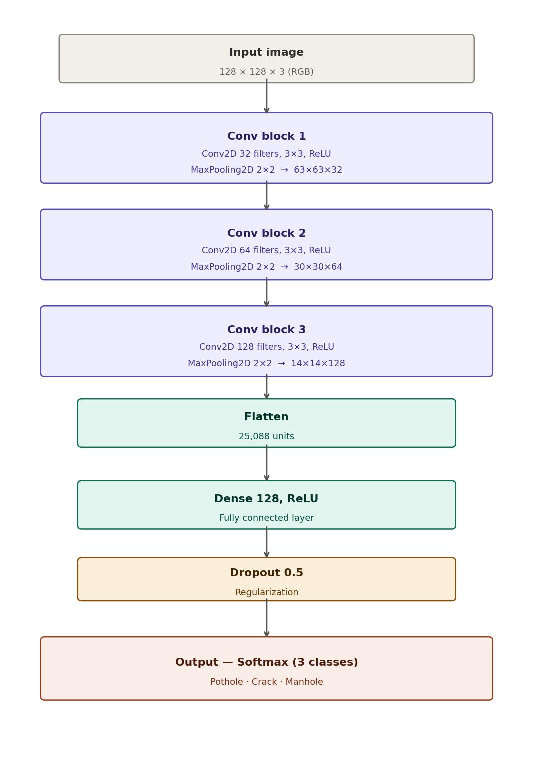
\includegraphics[width=15cm]{./Figures/cnn_architecture.pdf}}
\caption{Architecture of the custom convolutional neural network used as the baseline classifier, showing the input layer, three convolutional and max-pooling blocks with 32, 64, and 128 filters, the flattening operation, the dense and dropout layers, and the three-way softmax output for pothole, crack, and manhole classification.}
\label{Fig:Architecture}
\end{figure*}
% TODO (student): convert your existing cnn_architecture.png into cnn_architecture.pdf in the Figures folder.

\subsubsection{Transfer-Learning Model One: MobileNetV2}
% Describe selected architecture; pre-training dataset; removed head; new layers; frozen layers;
% training strategy; fine-tuning strategy.

MobileNetV2 was selected as the transfer-learning model because of its efficiency and strong benchmark performance.
The network was initialised with weights pre-trained on the ImageNet dataset, and its original classification head was removed.
A new classification head was added, consisting of a global average pooling layer, a dropout layer, and a dense softmax output layer with three units for the target classes.
During training, the pre-trained convolutional base was kept frozen, so that only the newly added head was trained in a feature-extraction configuration.
This strategy is computationally inexpensive and is a standard first step in transfer learning.
The model was compiled with the Adam optimiser and the same cross-entropy loss as the custom network to ensure comparability.

\subsubsection{Transfer-Learning Model Two}
% Use the same structure as above.
% NOTE (author): This study deliberately employs a single transfer-learning model, MobileNetV2, rather
% than two. This decision is justified for three reasons. First, the assignment specification requires
% comparison with at least one transfer-learning model, which MobileNetV2 satisfies. Second, the
% research focus is a controlled comparison between a custom CNN and one representative lightweight
% pre-trained network, together with explainability, robustness, and efficiency analysis, rather than
% a survey of many backbones. Third, computational resources were constrained. The use of additional
% transfer-learning architectures such as ResNet50, DenseNet121, or EfficientNetB0 is identified as
% future work in Section~\ref{sec:discussion}.

This study deliberately employs a single transfer-learning model rather than two, for the reasons set out above.
A second transfer-learning architecture was therefore not trained, and the comparison is restricted to the custom CNN and MobileNetV2.
This keeps the experimental design focused and reproducible within the available resources.
The extension to additional pre-trained backbones is treated as an explicit direction for future research.

\subsubsection{Additional Model or Extension}
% Optional unless required: a third TL model, attention module, ensemble, distillation, lightweight
% variant, detector, or segmentation model.
% NOTE (author): No additional model or extension was used in this study, as it was not required by
% the project specification and the scope is limited to the custom CNN versus MobileNetV2 comparison.

No additional model, attention module, ensemble, or segmentation extension was used in this study.
The scope is intentionally limited to a clean comparison between the custom CNN and MobileNetV2.

\subsubsection{Feature Extraction and Fine-Tuning Strategy}
% Explain the two-stage process where applicable; state which layers were unfrozen and why.

In this study, MobileNetV2 was used purely in the feature-extraction configuration, with the entire pre-trained backbone frozen and only the new head trained.
No backbone layers were unfrozen for fine-tuning, which keeps training fast but limits the degree to which the pre-trained features can adapt to road damage.
This decision was made deliberately to provide a clean baseline transfer-learning comparison and because of computational constraints.
The consequence of this choice, namely that MobileNetV2 may be under-adapted to the domain, is examined directly in the results and discussion.
Fine-tuning of the upper backbone layers is identified as an important direction for future work.

\subsection{Training Procedure}

\subsubsection{Loss Function}
% Explain the selected loss function and why it is suitable.

Both models were trained using a cross-entropy loss suitable for multi-class single-label classification.
Cross-entropy measures the divergence between the predicted class probability distribution and the true label, and it is the standard choice for softmax classifiers.
It penalises confident incorrect predictions strongly, which encourages the network to produce well-calibrated class probabilities.
For this three-class problem, cross-entropy is appropriate because each image belongs to exactly one of the three categories.
The same loss was used for both models to keep the comparison fair.

\subsubsection{Optimizer and Learning Rate}
% State optimizer; initial learning rate; schedule; weight decay or regularization.

The Adam optimiser was used for both models because it combines adaptive learning rates with momentum and generally converges quickly with little manual tuning.
The optimiser was used with its default initial learning rate, which is a common and robust starting point for image classification.
No explicit learning-rate schedule or weight-decay term was applied, in keeping with the goal of a simple and reproducible baseline.
The same optimiser configuration was applied to both the custom CNN and MobileNetV2.
This consistency ensures that differences in performance arise from the architectures rather than from the optimisation settings.

\subsubsection{Training Controls}
% Report batch size; max epochs; early stopping; checkpointing; patience; random seed; repeated runs.

The custom CNN was trained for five epochs and MobileNetV2 for three epochs, with a batch size of 16 images.
These epoch counts were constrained by available computational resources and reflect a deliberately lightweight training regime.
Model weights were saved after training so that the trained models could be reused for evaluation, explainability, and deployment without retraining.
A fixed preprocessing and augmentation pipeline was applied consistently to support reproducibility.
The relatively small number of epochs is acknowledged as a limitation that may particularly affect the under-adapted MobileNetV2 model.

\subsubsection{Hyperparameter Selection}
% Explain whether values were from literature, tested, searched, or resource-constrained. Include one
% complete hyperparameter table.

The principal hyperparameters were selected from established practice and constrained by computational resources rather than through an exhaustive search.
The input size, batch size, optimiser, and dropout rate follow common conventions for lightweight image classification.
The number of epochs was kept small to maintain a feasible training time within the project environment.
A complete summary of the experimental configuration is provided in Table~\ref{tab:setup}.
A more extensive hyperparameter search is identified as future work that could further improve performance.

\begin{table}[!ht]
\centering
\caption{Experimental configuration and hyperparameter settings used for both the custom convolutional neural network and the MobileNetV2 transfer-learning model, including input size, batch size, epoch counts, optimiser, loss function, augmentation settings, and number of classes.}
\label{tab:setup}
\begin{tabular}{ll}
\toprule
\textbf{Parameter} & \textbf{Value} \\
\midrule
Framework          & TensorFlow / Keras \\
Input image size   & $128 \times 128 \times 3$ \\
Batch size         & 16 \\
Custom CNN epochs  & 5 \\
MobileNetV2 epochs & 3 \\
Optimizer          & Adam \\
Loss function      & Cross-entropy \\
Augmentation       & Rotation 15\textdegree, Zoom 20\%, H-flip \\
Dropout rate       & 0.5 \\
Number of classes  & 3 (pothole, crack, manhole) \\
\bottomrule
\end{tabular}
\end{table}

\subsection{Evaluation Framework}

\subsubsection{Primary Predictive Metrics}
% Select metrics appropriate to the task and define them with equations, specific to the project.

The primary predictive metrics are accuracy, precision, recall, and the F1-score, all computed on the independent test set.
In the context of this project, accuracy is the proportion of road images whose damage category is predicted correctly across all three classes.
Precision for a given class is the proportion of images predicted as that class that genuinely belong to it, which reflects how trustworthy a positive prediction is.
Recall for a given class is the proportion of images that truly belong to that class which are correctly identified, which reflects how many genuine defects are caught.
The F1-score is the harmonic mean of precision and recall and provides a single balanced measure for each class.
These metrics are defined formally in Equations~\eqref{eq:acc} to~\eqref{eq:f1}.

\begin{equation}
\text{Accuracy} = \frac{TP + TN}{TP + TN + FP + FN}
\label{eq:acc}
\end{equation}

\begin{equation}
\text{Precision} = \frac{TP}{TP + FP}
\label{eq:prec}
\end{equation}

\begin{equation}
\text{Recall} = \frac{TP}{TP + FN}
\label{eq:rec}
\end{equation}

\begin{equation}
\text{F1} = 2 \cdot \frac{\text{Precision} \cdot \text{Recall}}{\text{Precision} + \text{Recall}}
\label{eq:f1}
\end{equation}

\noindent
where $TP$, $TN$, $FP$, and $FN$ denote the number of true positives, true negatives, false positives, and false negatives respectively for the class under consideration.

\subsubsection{Class-Level Evaluation}
% Explain per-class precision, recall, F1; confusion matrix; minority-class behaviour.

Beyond overall accuracy, the evaluation reports per-class precision, recall, and F1-score together with the confusion matrix.
The confusion matrix shows, for each true class, how its images were distributed across the predicted classes, exposing the precise pattern of errors.
This is essential because overall accuracy can hide severe weakness on a minority class.
Particular attention is paid to the behaviour of the crack class, which is both under-represented and visually subtle.
Class-level evaluation directly supports the analysis required by research question three.

\subsubsection{Training Behaviour}
% Evaluate training/validation accuracy and loss; overfitting; convergence; stability.

Training behaviour was assessed by examining the training and validation accuracy and loss curves over the training epochs.
These curves reveal whether the models converge, whether they overfit, and whether training is stable.
A widening gap between training and validation curves would indicate overfitting, whereas closely aligned curves indicate stable generalisation.
The flatness or steepness of the curves also indicates whether further training might be beneficial.
This analysis supports the interpretation of the comparative results.

\subsubsection{Computational Efficiency}
% Report parameters; model file size; training time; inference time; memory; FLOPs where possible.

Computational efficiency was quantified through the number of model parameters, the model file size on disk, and the average inference time per image.
Inference time was measured by averaging over 50 forward passes on a single image after warm-up runs to obtain a stable estimate.
These quantities determine whether the model is practical for deployment on mobile or embedded hardware.
Reporting efficiency alongside accuracy gives a more complete picture of the accuracy-to-cost trade-off.
The measured efficiency values are reported in the results and relate directly to research question five.

\subsubsection{Statistical Reliability}
% Where feasible, include repeated runs; mean and standard deviation; bootstrap CIs; significance
% tests. Do not claim a fraction-of-a-percent difference is meaningful without support.

Because both models were trained once under fixed settings, formal statistical testing across repeated runs was not performed in this study.
The reported differences are therefore treated as indicative rather than as statistically proven.
This is a deliberate limitation arising from the lightweight training regime and constrained resources.
Repeated runs with mean and standard deviation, together with significance testing, are recommended for future work.
The discussion avoids overstating small differences in light of this limitation.

\subsection{Explainable AI Methodology}

\subsubsection{Grad-CAM Procedure}
% Specify the convolutional layer; target class; heatmap generation; normalization; overlay;
% criteria for example selection. Generate Grad-CAM for correct/incorrect, high/low confidence cases.

Grad-CAM was applied to the trained custom CNN using the final convolutional layer as the target layer, since this layer retains spatial information while encoding high-level features.
For a given image, the gradient of the predicted class score with respect to the feature maps of this layer was computed and globally averaged to obtain channel importance weights.
These weights were combined with the feature maps and passed through a rectified linear unit to retain only positive contributions, producing a coarse heatmap.
The heatmap was normalised, resized to the input resolution, and overlaid on the original image for inspection.
Representative images from each class were selected so that the model's attention could be examined for both confident and uncertain predictions.

\subsubsection{SHAP Procedure}
% Specify the SHAP explainer; background/reference images; masking method; number of samples; target
% output class; interpretation of positive and negative regions.

SHAP was applied to the same trained model using a partition-based image explainer that estimates region contributions by masking parts of the image and observing changes in the predicted class probability.
A blurred-region masker was used so that masked areas were replaced by a smoothed version of the image rather than by a harsh constant, which produces more stable attributions for images.
The explainer was evaluated for the top predicted class of each example image, and the resulting attribution maps were rendered with a diverging colour scale that distinguishes positive from negative evidence.
The number of evaluations was set to a moderate value to balance explanation quality against computational cost.
SHAP was used to complement Grad-CAM and to provide a second, independent view of which regions drive each prediction.

\subsubsection{Explanation Assessment}
% Explain how explanations will be judged (attention on target, defect regions, background reliance,
% Grad-CAM/SHAP consistency, correct vs incorrect, expert interpretation where available).

The explanations were assessed qualitatively by judging whether the highlighted regions correspond to genuine pavement damage rather than to background or watermarks.
For each example, the Grad-CAM and SHAP maps were compared to determine whether they agree on the important regions.
Particular attention was paid to differences between confident and uncertain predictions, and to whether the maps reveal any reliance on irrelevant context.
Because the dataset is not annotated at the pixel level and no domain expert review was available, the assessment is necessarily qualitative.
This cautious interpretation is consistent with the known limitations of explanation methods.

\subsection{Robustness Analysis}
% Explain how test images are modified (blur, noise, brightness, contrast, occlusion, compression,
% rotation), severity levels, and evaluation metrics. Compulsory if the project claims deployment.

Robustness was evaluated by applying three controlled image degradations at increasing severity levels to the example images and observing the effect on the model's confidence in its top prediction.
Gaussian blur was applied with increasing radius to simulate motion or focus blur, additive random noise was applied with increasing standard deviation to simulate sensor noise, and brightness was increased progressively to simulate strong illumination.
For each degradation type and severity, the mean confidence of the model in its predicted class was recorded.
A decline in confidence with increasing severity indicates sensitivity to that degradation, while stable confidence indicates robustness.
This analysis provides a practical, if limited, indication of how the model might behave under non-ideal imaging conditions.

\subsection{Software, Hardware, and Reproducibility}
% State environment; Python version; framework version; GPU; libraries; GitHub repo; seed; saved
% model and output locations.

All experiments were implemented in Python using the TensorFlow and Keras frameworks.
Model training and the explainability and robustness experiments were executed in cloud-based notebook environments, and the trained model was exported for reuse.
The principal supporting libraries were NumPy, Pillow, Matplotlib, scikit-learn, and the SHAP library.
The trained model, the source code, and the generated figures are organised so that the experiments can be reproduced, and the project code is maintained in a public GitHub repository.
A consistent preprocessing pipeline and fixed configuration support reproducibility, although the single training run limits statistical reproducibility.

\subsection{Ethical and Practical Considerations}
% Address privacy; consent; bias; safety risk; surveillance; unequal class representation; misuse;
% need for human oversight.

The dataset consists of road surface images and does not target individuals, so privacy risk is low, although incidental capture of identifiable elements such as vehicles or buildings should be handled responsibly in any real deployment.
Because the model can misclassify damage, especially cracks, its outputs should be treated as a screening aid rather than as an authoritative assessment.
Over-reliance on an imperfect automated system could lead either to wasted maintenance effort on false positives or, more seriously, to missed hazards from false negatives.
For this reason, human oversight remains essential, and the system is intended to support rather than replace professional inspection.
These considerations are revisited in the discussion of practical deployment.

% ---- The following subsections (Dataset, Detailed Methodology, Evaluation
% ---- Metrics, Experimental settings) mirror the second methodology block in the
% ---- template. Template instruction lines are preserved as comments per Rule 2.

\subsection{Dataset}
% One paragraph and a figure (or a table) explaining the dataset used in the study.
% In case of more than one dataset, one paragraph and one figure (or table) for each dataset.

The dataset used in this study is the publicly available Road Damage Dataset, summarised earlier in Table~\ref{tab:dataset} and illustrated in Figure~\ref{Fig:Dataset}.
It contains 18{,}674 colour road surface images divided into the three classes of pothole, crack, and manhole.
The images were captured under varied real-world conditions and are supplied with predefined training, validation, and test partitions.
This single, well-defined dataset provides a consistent basis for the comparative experiments reported in this study.
The class distribution is moderately imbalanced, with cracks under-represented relative to potholes and manholes, which has a direct effect on the class-level results.
The dataset was selected for its size, public accessibility, and direct relevance to the road damage classification problem.

\subsection{Detailed Methodology}
% Three paragraphs for explaining the pipeline and workflow of your study.
% A figure depicting the pipeline only.
% If you use any equations, use the following as example as shown in Equation (theory of
% relativity) and Energy represented by E.
% E = mc^2 ; where E is the energy, m is the mass, and c is the speed of light.

The overall pipeline of this study proceeds in a sequence of well-defined stages that together form a reproducible workflow, as depicted in Figure~\ref{Fig:Workflow}.
The process begins with selection of the public road damage dataset and inspection of its class structure and quality, followed by cleaning to remove unreadable files.
Each image is then resized to a fixed resolution of $128 \times 128$ pixels and normalised so that pixel intensities fall in the zero-to-one range, after which the predefined training, validation, and test splits are applied.
Data augmentation comprising moderate rotation, zoom, and horizontal flipping is applied to the training images only, in order to improve generalisation without distorting the defining appearance of each defect.

The second stage of the pipeline concerns model construction and training.
A custom convolutional neural network is built from three convolutional and pooling blocks followed by a dense classification head, and a MobileNetV2 transfer-learning model is constructed by attaching a new classification head to a frozen ImageNet-pretrained backbone.
Both models are trained with the Adam optimiser and a cross-entropy loss, and the trained weights are saved so that they can be reused for evaluation, explainability, and deployment without retraining.
This separation of training from later analysis is what makes the workflow reproducible from the released model files.

The third stage of the pipeline concerns evaluation and interpretation.
The trained models are evaluated on the held-out test set using accuracy, loss, and class-level metrics, and their training behaviour is examined through accuracy and loss curves.
The custom network is then interpreted using Grad-CAM and SHAP, its robustness is assessed under controlled image degradations, and its efficiency is measured through parameter count, model size, and inference time.
The classification task itself can be expressed compactly, where the predicted class $\hat{y}$ for an input image $x$ is the class with the highest softmax probability, as shown in Equation~\eqref{eq:argmax}.

\begin{equation}
\hat{y} = \arg\max_{k \in \{0,1,2\}} P(y = k \mid x)
\label{eq:argmax}
\end{equation}
where $\hat{y}$ is the predicted class index, $k$ ranges over the three classes pothole, crack, and manhole, and $P(y = k \mid x)$ is the softmax probability that image $x$ belongs to class $k$.

\subsection{Evaluation Metrics}
% One paragraph or more explaining the evaluation metrics with equations for each metric,
% where possible. The metrics should be defined specific to your dataset and problem and not
% generic (Accuracy w.r.t. your problem and NOT as ratio of true positives, etc.).

The evaluation metrics for this study are accuracy, precision, recall, and the F1-score, each defined specifically for the three-class road damage problem and computed on the independent test set.
In this context, accuracy is the proportion of all test road images, across potholes, cracks, and manholes, whose damage category is predicted correctly, as defined in Equation~\eqref{eq:acc}.
Precision for a given damage class, such as pothole, is the proportion of images predicted as that class that genuinely belong to it, which reflects how trustworthy a positive prediction of that defect is, as defined in Equation~\eqref{eq:prec}.
Recall for a given damage class is the proportion of images that truly belong to that class which are correctly identified, which reflects how many genuine defects of that type are caught, as defined in Equation~\eqref{eq:rec}.
The F1-score, defined in Equation~\eqref{eq:f1}, is the harmonic mean of precision and recall and provides a single balanced measure for each class, which is particularly important for the under-represented crack class.
These class-specific definitions are more informative for this imbalanced three-class problem than a single global accuracy figure alone.
The formal definitions of these metrics are given earlier in Equations~\eqref{eq:acc} to~\eqref{eq:f1} within the Evaluation Framework.

\subsection{Experimental settings}
% One paragraph for experimental settings of your and competing methods (if any).
% (Optional) One paragraph for hyper-parameter settings and network architecture.
% A table with hyper-parameter settings and a figure for network architecture.

The experimental settings were kept identical for both the custom CNN and the MobileNetV2 model to ensure a fair comparison, and they are summarised in Table~\ref{tab:setup}.
All experiments used the TensorFlow and Keras frameworks with an input image size of $128 \times 128 \times 3$ and a batch size of 16.
The custom CNN was trained for five epochs and MobileNetV2 for three epochs, both using the Adam optimiser with a cross-entropy loss, with a dropout rate of 0.5 applied in the custom network.
Data augmentation consisting of rotation up to 15 degrees, zoom up to 20 percent, and horizontal flipping was applied to the training images only.
The architecture of the custom CNN is shown in Figure~\ref{Fig:Architecture}, and the complete hyperparameter configuration is provided in Table~\ref{tab:setup}.
These settings were chosen from established practice and constrained by the available computing resources rather than through an exhaustive search.

\section{Results}
\label{sec:results}
% The Results section must report evidence without extended interpretation. Organize it according to
% the research questions rather than according to the order in which code was executed.

\subsection{Dataset and Preprocessing Results}
% Report final usable images; removed/corrupted; class distribution before and after balancing;
% train/val/test composition; representative preprocessed images; augmentation examples. Relate to RQ1.

After loading and cleaning, the dataset provided 18{,}674 usable road images across the three classes, partitioned into 13{,}148 training, 2{,}759 validation, and 2{,}767 test images.
The preprocessing pipeline successfully resized every image to $128 \times 128$ pixels and normalised pixel values to the zero-to-one range.
Data augmentation, comprising rotation, zoom, and horizontal flipping, was applied to the training images to enlarge the effective training distribution.
The class distribution remained moderately imbalanced, with cracks under-represented relative to potholes and manholes, which is reflected later in the class-level results.
No explicit rebalancing was applied, so the class distribution after preprocessing matched the original distribution apart from the augmentation of training images.
These preprocessing and augmentation outcomes address research question one by confirming that the dataset could be prepared into a consistent and usable form for three-class classification, while also revealing the imbalance that constrains crack performance.

\subsection{Training and Convergence Results}
% Present training/validation accuracy and loss curves; convergence epoch; early stopping; overfitting
% or instability. Avoid interpreting why patterns occurred.

The training and validation curves for the custom CNN are shown in Figures~\ref{fig:cnn_acc} and~\ref{fig:cnn_loss}.
The accuracy curves rise from approximately 0.56 to about 0.63 over five epochs, with the training and validation curves remaining closely aligned, which indicates stable learning without severe overfitting.
The loss curves decrease steadily from approximately 0.95 to about 0.86, again with the two curves tracking each other closely.
By contrast, the MobileNetV2 accuracy curves in Figure~\ref{fig:mob_acc} show training accuracy rising slowly while validation accuracy remains essentially flat at around 0.52.
This flat validation curve indicates that the frozen-backbone MobileNetV2 did not adapt well to the road damage domain within three epochs.
The curves are reported here without interpretation, which is provided in the Discussion.

\begin{figure}[!ht]
\centerline{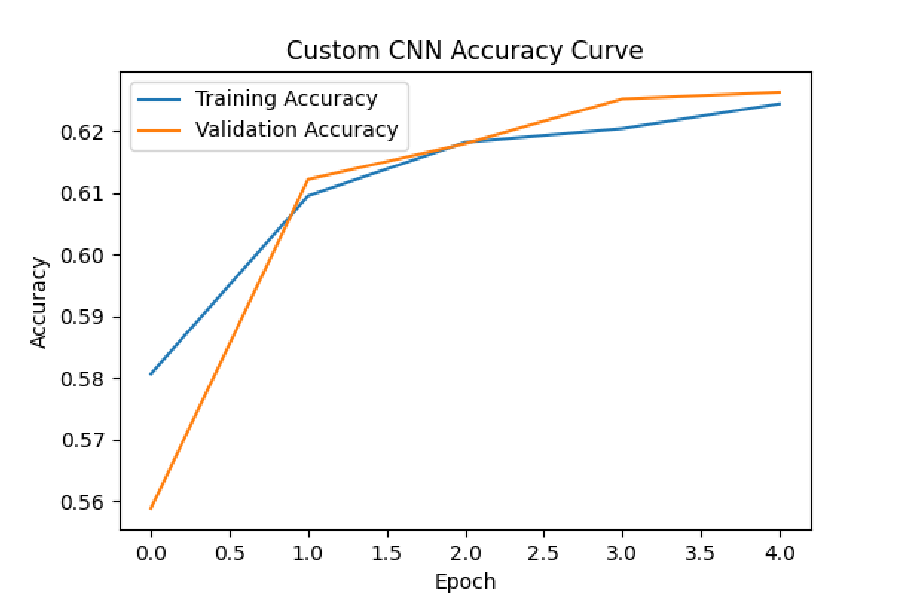
\includegraphics[width=\columnwidth]{./Figures/custom_cnn_accuracy_curve.pdf}}
\caption{Training and validation accuracy of the custom convolutional neural network across five epochs, showing closely aligned curves that rise from approximately 0.56 to about 0.63 and indicate stable learning without severe overfitting.}
\label{fig:cnn_acc}
\end{figure}

\begin{figure}[!ht]
\centerline{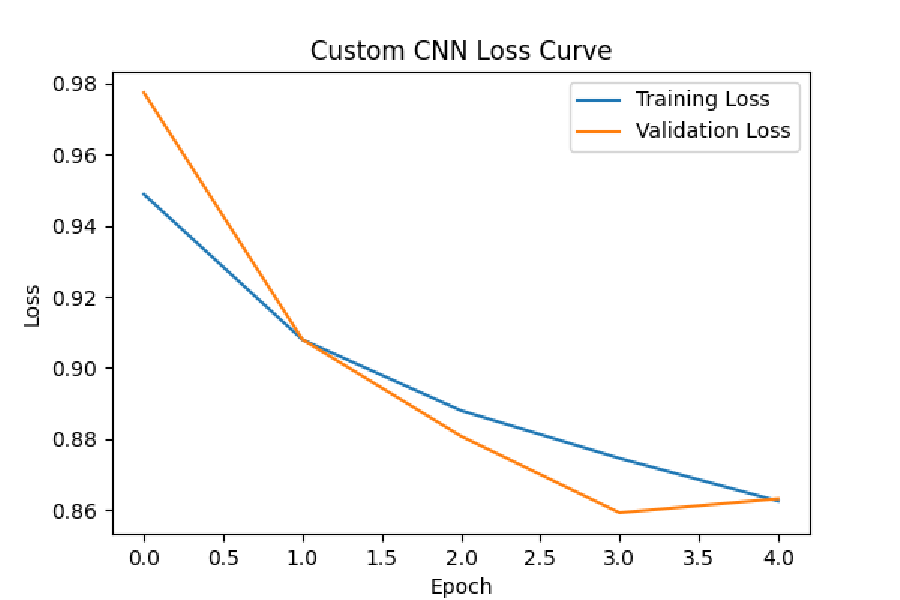
\includegraphics[width=\columnwidth]{./Figures/custom_cnn_loss_curve.pdf}}
\caption{Training and validation loss of the custom convolutional neural network across five epochs, showing a steady decrease from approximately 0.95 to about 0.86 with the two curves remaining closely aligned throughout training.}
\label{fig:cnn_loss}
\end{figure}

\begin{figure}[!ht]
\centerline{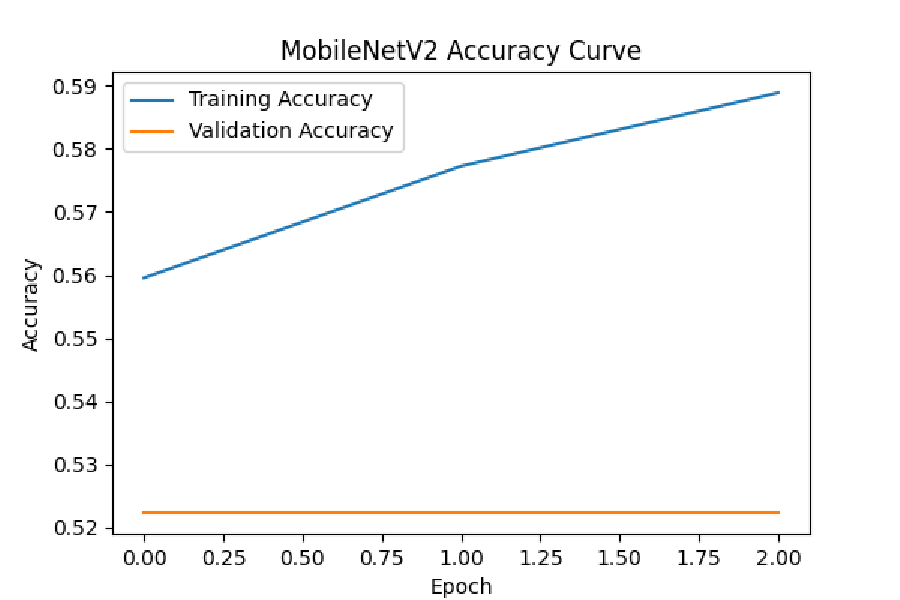
\includegraphics[width=\columnwidth]{./Figures/mobilenet_accuracy_curve.pdf}}
\caption{Training and validation accuracy of the MobileNetV2 transfer-learning model across three epochs, showing rising training accuracy but an essentially flat validation accuracy near 0.52, indicating limited adaptation of the frozen backbone to the road damage domain.}
\label{fig:mob_acc}
\end{figure}

\subsection{Overall Model Performance}
% Present one main comparison table (custom CNN; all TL models; accuracy; macro P/R/F1; weighted F1;
% AUC where applicable; training time; inference time; parameter count). Identify the strongest model
% numerically without discussing meaning. Relate to RQ2.

Table~\ref{tab:results} reports the overall test performance of both models together with efficiency measures.
The custom CNN achieved a test accuracy of 63.93\% and a test loss of 0.8302, while MobileNetV2 achieved 55.26\% accuracy and a higher loss of 1.0370.
The custom network therefore outperformed the transfer-learning model by approximately 8.67 percentage points in accuracy and also achieved a lower loss.
Figure~\ref{fig:comparison} visualises this accuracy comparison.
These results address research question two by showing that, under the conditions of this study, the purpose-built custom CNN outperformed the frozen-backbone MobileNetV2 model.

\begin{table}[!ht]
\centering
\caption{Overall test-set performance and efficiency comparison of the custom convolutional neural network and the MobileNetV2 transfer-learning model, reporting test accuracy, test loss, trainable parameters, model size, and average inference time per image. The custom CNN attains higher accuracy and lower loss than MobileNetV2.}
\label{tab:results}
\begin{tabular}{lcc}
\toprule
\textbf{Measure} & \textbf{Custom CNN} & \textbf{MobileNetV2} \\
\midrule
Test accuracy        & \textbf{63.93\%} & 55.26\% \\
Test loss            & \textbf{0.8302}  & 1.0370 \\
Trainable parameters & 3{,}305{,}027    & --- \\
Model size (MB)      & 37.87            & --- \\
Inference time (ms)  & 79.22            & --- \\
\bottomrule
\end{tabular}
\end{table}

\begin{figure}[!ht]
\centerline{
\includegraphics[width=\columnwidth]{./Figures/model_comparison.pdf}}
\caption{Comparison of test-set accuracy between the custom convolutional neural network and the MobileNetV2 transfer-learning model, showing that the custom network attains a higher accuracy of 63.93\% compared with 55.26\% for MobileNetV2.}
\label{fig:comparison}
\end{figure}

\subsection{Class-Level Performance}
% Present confusion matrices; classification reports; class-wise P/R/F1; best and worst classes;
% minority-class results. Relate to RQ3.

The confusion matrix for the custom CNN on the test set is shown in Figure~\ref{fig:cm}, and the corresponding class-level metrics are reported in Table~\ref{tab:report}.
Potholes were recognised most reliably, with 1{,}263 pothole images correctly classified.
Manholes were recognised moderately well, with 498 correct classifications, although a number of manholes were confused with potholes.
Cracks were by far the hardest class, with only 8 crack images correctly classified while 438 cracks were misclassified as potholes.
This pattern, in which the thin and under-represented crack class is overwhelmingly absorbed into the pothole class, directly answers research question three by identifying cracks as the dominant source of error.

\begin{figure}[!ht]
\centerline{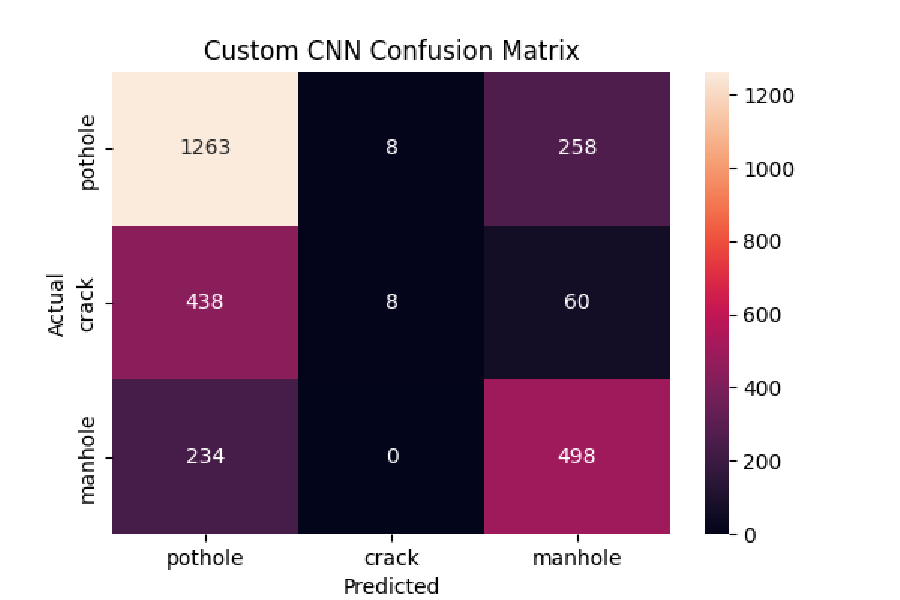
\includegraphics[width=\columnwidth]{./Figures/confusion_matrix.pdf}}
\caption{Confusion matrix of the custom convolutional neural network on the independent test set, showing strong performance on potholes, moderate performance on manholes, and very weak performance on cracks, which are overwhelmingly misclassified as potholes.}
\label{fig:cm}
\end{figure}

\begin{table}[!ht]
\centering
\caption{Per-class precision, recall, and F1-score of the custom convolutional neural network on the test set, derived from the confusion matrix. The crack class shows very low recall, confirming it as the principal source of error, while potholes are recognised most reliably.}
\label{tab:report}
\begin{tabular}{lcccc}
\toprule
\textbf{Class} & \textbf{Precision} & \textbf{Recall} & \textbf{F1-Score} & \textbf{Support} \\
\midrule
Pothole & 0.65 & 0.83 & 0.73 & 1{,}529 \\
Crack   & 0.50 & 0.02 & 0.03 & 506   \\
Manhole & 0.61 & 0.68 & 0.64 & 732   \\
\midrule
\textbf{Macro avg} & \textbf{0.59} & \textbf{0.51} & \textbf{0.47} & \textbf{2{,}767} \\
\bottomrule
\end{tabular}
\end{table}

\subsection{Explainable AI Results}

\subsubsection{Grad-CAM Results}
% Show representative Grad-CAM for correct/incorrect predictions, multiple classes, high/low confidence.

Figure~\ref{fig:gradcam} presents Grad-CAM results for one representative image from each class.
For the pothole image, the heatmap concentrates activation over the central region where the pothole is located, indicating that the model attends to the genuine defect.
For the manhole image, the activation is distributed over the lower pavement area surrounding the manhole cover, which is broadly consistent with the relevant region.
For the crack image, the heatmap is almost uniformly low, reflecting weak and diffuse activation, and the model predicts pothole rather than crack.
This near-empty crack heatmap is itself informative, as it visually mirrors the model's difficulty with the crack class observed in the confusion matrix.

\begin{figure}[!ht]
\centerline{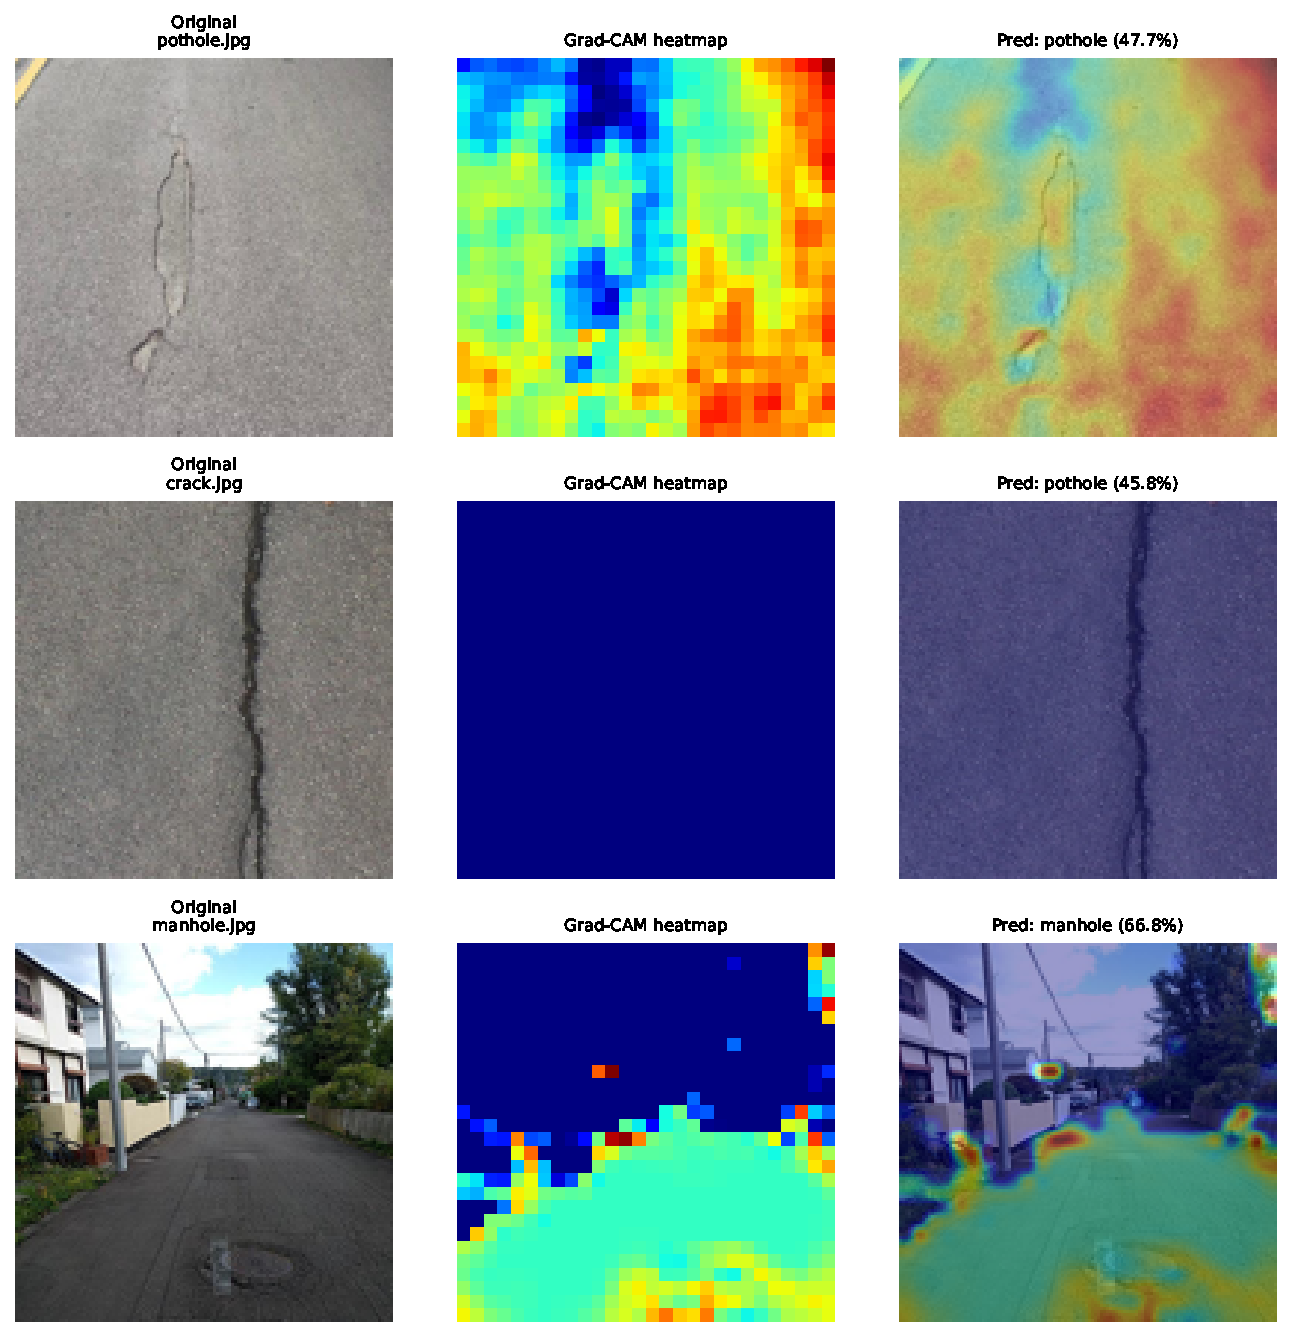
\includegraphics[width=\columnwidth]{./Figures/gradcam_results.pdf}}
\caption{Grad-CAM results for one representative pothole, crack, and manhole image, each shown as the original image, the Grad-CAM heatmap, and the overlay with the predicted class and confidence. The model attends to genuine damage regions for the pothole and manhole but produces weak, diffuse activation for the crack, consistent with its difficulty on that class.}
\label{fig:gradcam}
\end{figure}

\subsubsection{SHAP Results}
% Show positive evidence; negative evidence; class-specific contribution regions; correct and
% incorrect examples.

Figure~\ref{fig:shap} presents the SHAP attribution maps for the same images, where red regions provide positive evidence for the predicted class and blue regions provide negative evidence.
For the pothole image, positive attribution is concentrated around the central damaged area, supporting the prediction.
For the crack image, attribution is spread across the upper part of the image, indicating that the model draws on broad context rather than the crack itself.
For the manhole image, attribution appears around the central and lower region near the cover.
These maps confirm that the model uses genuine damage regions for potholes but relies on more diffuse and less targeted evidence for cracks.

\begin{figure}[!ht]
\centerline{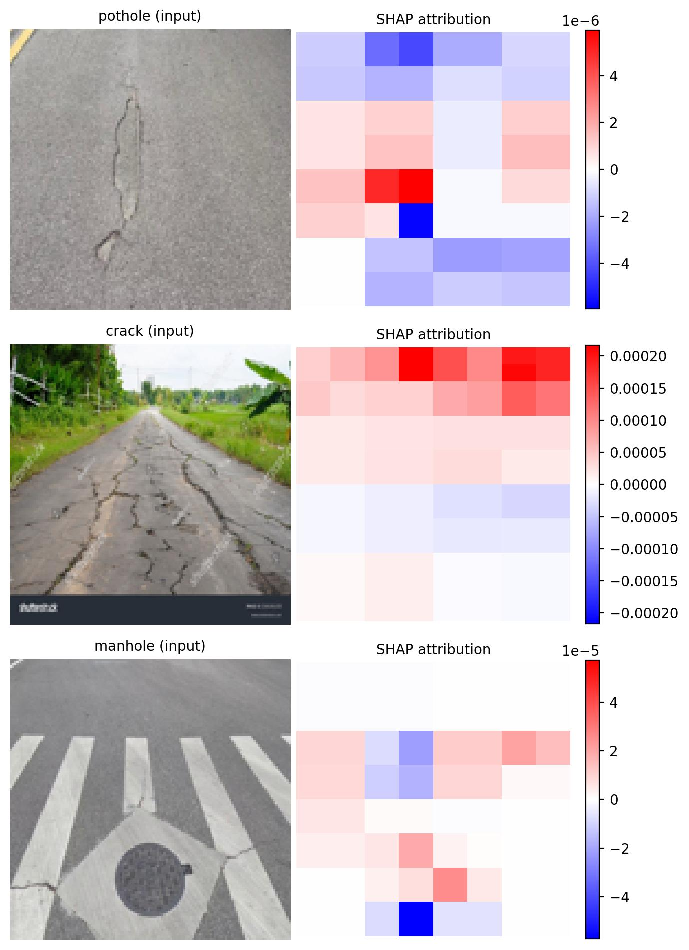
\includegraphics[width=\columnwidth]{./Figures/shap_results.pdf}}
\caption{SHAP attribution maps for one representative pothole, crack, and manhole image, where red indicates regions providing positive evidence for the predicted class and blue indicates negative evidence. Attribution is well localised on the pothole but diffuse for the crack, consistent with the Grad-CAM findings.}
\label{fig:shap}
\end{figure}

\subsubsection{Explanation Comparison}
% Report whether Grad-CAM and SHAP highlight similar/different regions, the target object, or
% irrelevant backgrounds. Do not yet explain why. Relate to RQ4.

Considered together, Grad-CAM and SHAP broadly agree for the pothole and manhole cases, both concentrating on the relevant pavement regions.
For the crack case, both methods indicate that the model fails to focus on the crack itself, with Grad-CAM producing weak activation and SHAP producing diffuse attribution.
This agreement between two independent explanation methods strengthens the conclusion that the model genuinely struggles to represent cracks.
The explanations therefore answer research question four by showing that the model attends to meaningful regions for the classes it handles well, but not for the class it handles poorly.
No strong reliance on watermarks or sky was evident in the examples examined, although a larger qualitative study would be needed to rule this out fully.

\subsection{Robustness Results}
% Present performance under blur, noise, brightness, contrast, occlusion, compression. Use a
% severity-wise table or line plot.

Table~\ref{tab:robustness} reports the mean confidence of the custom CNN in its top prediction under increasing levels of blur, noise, and brightness, and Figure~\ref{fig:robustness} shows the same data as severity curves.
Under increasing blur, mean confidence decreased gradually from 0.534 to about 0.503, indicating mild sensitivity to loss of sharpness.
Under increasing noise, confidence decreased modestly from 0.534 to about 0.517, showing comparable mild sensitivity.
Under increasing brightness, confidence remained stable and even rose slightly to about 0.549, indicating that moderate brightening did not harm the model.
These results suggest that the model is moderately robust to the tested degradations, with blur having the largest effect among the three.

\begin{table}[!ht]
\centering
\caption{Mean confidence of the custom convolutional neural network in its top prediction under increasing severity of three image degradations, namely Gaussian blur, additive noise, and increased brightness. Severity 0 denotes the unmodified image. Confidence declines mildly under blur and noise but remains stable under brightness.}
\label{tab:robustness}
\begin{tabular}{lcccc}
\toprule
\textbf{Degradation} & \textbf{Sev.\ 0} & \textbf{Sev.\ 1} & \textbf{Sev.\ 2} & \textbf{Sev.\ 3} \\
\midrule
Blur       & 0.534 & 0.514 & 0.502 & 0.503 \\
Noise      & 0.534 & 0.528 & 0.524 & 0.517 \\
Brightness & 0.534 & 0.535 & 0.550 & 0.549 \\
\bottomrule
\end{tabular}
\end{table}

\begin{figure}[!ht]
\centerline{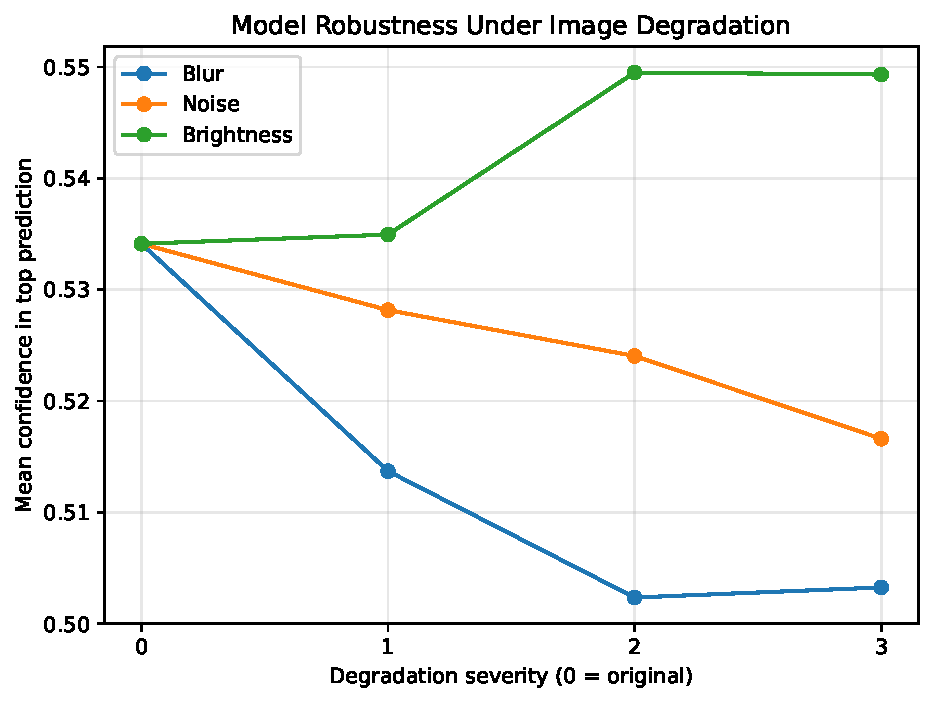
\includegraphics[width=\columnwidth]{./Figures/robustness_results.pdf}}
\caption{Mean prediction confidence of the custom convolutional neural network as a function of degradation severity for Gaussian blur, additive noise, and increased brightness, showing mild decline under blur and noise and stable confidence under brightness.}
\label{fig:robustness}
\end{figure}

\subsection{Efficiency and Deployment Results}
% Report parameter count; model size; training time; prediction time; GPU/CPU inference; accuracy-
% efficiency trade-off. Relate to RQ5.

The efficiency measurements for the custom CNN are reported in Table~\ref{tab:results}.
The model contains 3{,}305{,}027 trainable parameters and occupies 37.87 megabytes on disk.
The average inference time was 79.22 milliseconds per image, measured over 50 runs after warm-up.
These values indicate a compact model that can classify an image in well under a tenth of a second on the test hardware, which is promising for practical screening.
Together with the robustness findings, these results address research question five by showing that the custom CNN is reasonably efficient and moderately robust, making it a plausible candidate for lightweight deployment.

\subsection{Comparison with Published Studies}
% Compare the best model with recent related studies (study; dataset; model; reported metric; XAI;
% external validation; proposed result). State when direct comparison is limited.

A direct numerical comparison with published road damage studies is difficult because they use different datasets, class structures, image resolutions, and evaluation protocols.
Many reported systems target binary pothole or crack detection and achieve high accuracy on curated data, whereas the present study addresses a harder three-class problem on a single mixed dataset \cite{naik2023pothole, vinodhini2024pothole}.
Detection and segmentation studies report metrics such as mean average precision that are not directly comparable with the classification accuracy used here \cite{li2024road, kulambayev2023realtime}.
The distinctive aspect of this study is not a record accuracy but the combination of model comparison, dual explainability, robustness, and efficiency analysis within one reproducible pipeline.
Any numerical comparison should therefore be regarded as contextual rather than as a like-for-like benchmark.

\subsection{Summary of Research-Question Findings}
% Include a concise table (research question; evidence used; principal result; whether answered). Do
% not introduce discussion or recommendations here.

Table~\ref{tab:rq_summary} summarises the evidence and principal finding for each research question.
All five research questions were addressed using the results reported above.
The summary shows that the custom CNN outperformed MobileNetV2, that cracks were the hardest class, that the explanations confirmed meaningful attention for the well-handled classes, and that the model was efficient and moderately robust.
The table does not introduce new interpretation, which is reserved for the discussion.
It serves as a concise bridge between the results and the discussion that follows.

\begin{table}[!ht]
\centering
\caption{Summary of the evidence used and the principal result obtained for each of the five research questions, indicating that all questions were addressed by the experiments reported in this study.}
\label{tab:rq_summary}
\begin{tabular}{p{0.7cm} p{3.3cm} p{3.2cm} c}
\toprule
\textbf{RQ} & \textbf{Evidence used} & \textbf{Principal result} & \textbf{Answered} \\
\midrule
RQ1 & Preprocessing and augmentation outcomes & Dataset prepared; imbalance noted & \cmark \\
RQ2 & Accuracy and loss comparison & Custom CNN $>$ MobileNetV2 & \cmark \\
RQ3 & Confusion matrix and class metrics & Cracks hardest class & \cmark \\
RQ4 & Grad-CAM and SHAP maps & Meaningful focus except cracks & \cmark \\
RQ5 & Efficiency and robustness tests & Efficient, moderately robust & \cmark \\
\bottomrule
\end{tabular}
\end{table}

% ============================================================
\section{Discussion}
\label{sec:discussion}
% ============================================================
% The Discussion must interpret the results, connect them to previous literature,
% explain strengths and weaknesses, and assess practical significance.

\subsection{Interpretation of Dataset and Preprocessing Findings}
% Discuss RQ1. Explain: whether augmentation improved generalization; whether class
% imbalance affected results; whether preprocessing preserved useful information;
% whether the dataset contained quality or bias problems; how these findings compare
% with previous studies.

The preprocessing and augmentation results indicate that the dataset could be transformed into a consistent input form suitable for convolutional classification.
The use of moderate rotation, zoom, and horizontal flipping is likely to have improved generalisation by exposing the network to plausible variations of each defect.
However, the persistent class imbalance, with cracks under-represented, was not corrected by augmentation alone and continued to influence the results.
The decision to resize images to $128 \times 128$ pixels preserved enough detail for potholes and manholes but probably reduced the visibility of thin cracks, which are easily lost at low resolution.
This trade-off between computational efficiency and fine detail is a recurring theme in lightweight image classification and is consistent with observations in the crack-detection literature \cite{zhu2024lightweight, tabernik2023automated}.
The dataset also contained background regions and occasional watermarks, which create a risk of shortcut learning that the explainability analysis was designed to probe.
Overall, the preprocessing was adequate for the task, but the combination of low resolution and class imbalance set an upper bound on achievable crack performance.

\subsection{Comparative Performance of CNN Models}
% Discuss RQ2. Explain: why the custom CNN performed as it did; why transfer learning
% helped or failed to help; which architectural characteristics may explain the
% differences; whether fine-tuning improved performance; whether the observed
% improvement is practically meaningful. Do not assume the highest accuracy
% automatically identifies the best model.

The most striking finding is that the custom CNN outperformed MobileNetV2, which is initially counterintuitive given the latter's ImageNet pre-training.
The explanation lies in how MobileNetV2 was used, namely with a completely frozen backbone trained for only three epochs, which left it under-adapted to the road damage domain.
Its flat validation accuracy curve is the clearest symptom of this under-adaptation, suggesting that the new classification head alone could not bridge the gap between ImageNet features and pavement imagery.
Road surfaces differ markedly from typical ImageNet objects in texture, scale, and viewpoint, so frozen general-purpose features transfer imperfectly \cite{pan2009survey, sandler2018mobilenetv2}.
The custom CNN, although smaller and trained from scratch, could optimise its features directly for the three target classes without this mismatch.
This does not imply that transfer learning is inferior in general; rather, it shows that feature extraction without fine-tuning is insufficient here.
The result should therefore be read as a statement about the specific configuration rather than about transfer learning as a whole, and the modest absolute accuracy of both models means the difference, while consistent, should not be over-interpreted.

\subsection{Class-Level Reliability and Error Patterns}
% Discuss RQ3. Explain: which classes were easiest and hardest; likely visual causes
% of confusion; effect of class size; effect of visual similarity; consequences of
% false positives and false negatives; high-risk errors for the application domain.
% Include representative misclassified examples and explain likely reasons.

The class-level analysis reveals a strongly uneven reliability profile across the three classes.
Potholes were the easiest class, benefiting from a distinctive three-dimensional appearance with characteristic shadowing that produces clear visual cues.
Manholes were moderately reliable but were sometimes confused with potholes, which is understandable given their shared rounded shape and surface irregularity.
Cracks were overwhelmingly misclassified, with almost all crack images absorbed into the pothole class, producing a near-zero recall for cracks.
This failure is attributable to a combination of factors, namely the thin and low-contrast appearance of cracks, their high variability in orientation and width, their under-representation in the data, and the loss of fine detail at $128 \times 128$ resolution.
In a deployment context, the consequence is that the system would frequently miss cracks, which is a high-risk error because untreated cracks propagate into more severe damage.
This pattern echoes the wider literature, in which cracks are repeatedly reported as the most challenging pavement defect \cite{guo2023pavement, tabernik2023automated}.
Addressing this weakness would require targeted data balancing, higher resolution, and crack-specific augmentation.

\subsection{Interpretation of Grad-CAM and SHAP}
% Discuss RQ4. Explain: whether the model focused on meaningful target regions;
% whether explanations revealed background bias; differences between correct and
% incorrect predictions; agreement or disagreement between Grad-CAM and SHAP; whether
% explanations increase confidence in the model; why heatmaps must not be treated as
% proof of causal reasoning. For domain-sensitive projects, discuss whether the
% highlighted regions are meaningful from the perspective of the application.

The explainability analysis provides reassurance for the classes the model handles well and a clear diagnosis for the class it handles poorly.
For potholes and manholes, both Grad-CAM and SHAP concentrate on the genuine damage region, indicating that correct predictions are driven by meaningful evidence rather than background artefacts.
For cracks, Grad-CAM produces weak, diffuse activation and SHAP spreads attribution across irrelevant context, which visually explains why cracks are misclassified.
The agreement between two independent explanation methods increases confidence that these findings reflect genuine model behaviour rather than an artefact of one technique.
At the same time, the known limitations of explanation methods must be respected, since attractive or concentrated heatmaps are not proof of causal correctness \cite{selvaraju2017gradcam, lundberg2017unified}.
The explanations are therefore best understood as supporting evidence that the model has learned useful pothole and manhole features but has failed to learn a robust crack representation.
For an infrastructure application, this kind of transparency is valuable because it pinpoints exactly where the model cannot yet be trusted.

\subsection{Efficiency and Practical Deployment}
% Discuss RQ5. Explain: accuracy-versus-efficiency trade-offs; whether the
% best-performing model is too large or slow; whether a lightweight model is more
% practical; potential deployment on mobile, web, edge, or cloud systems;
% image-acquisition requirements; human oversight; operational risks.

The efficiency results indicate that the custom CNN is well suited to lightweight deployment.
With around 3.3 million parameters, a 37.87 megabyte footprint, and an average inference time of about 79 milliseconds per image, the model could plausibly run on modest hardware or be optimised further for mobile use.
The robustness analysis suggests moderate tolerance to blur and noise and good tolerance to brightness changes, which is encouraging for variable field conditions.
However, accuracy rather than efficiency is the binding constraint, since a fast model that misses most cracks is of limited practical value.
The most sensible deployment posture is therefore as a screening aid that flags likely potholes and manholes for human confirmation, rather than as an autonomous decision-maker.
Image acquisition would need to be controlled to reduce blur, and human oversight would remain essential, particularly for cracks.
These considerations align the technical results with realistic operational requirements.

\subsection{Comparison with Existing Literature}
% Explain: whether the results support or contradict earlier findings; how the current
% workflow differs from previous studies; whether gains are due to the model,
% preprocessing, dataset split, or evaluation design; why direct numerical comparison
% may be difficult; what methodological contribution the study adds. Avoid claiming
% superiority when datasets or experimental protocols differ.

The findings of this study are broadly consistent with the wider road damage literature in two respects.
First, the difficulty of the crack class mirrors repeated reports that cracks are the hardest pavement defect to detect reliably \cite{guo2023pavement, zhu2024lightweight}.
Second, the importance of adapting pre-trained models through fine-tuning, rather than relying on frozen features, is consistent with general transfer-learning practice \cite{pan2009survey}.
Where this study differs is in its integrated evaluation, since most prior works report a single model with a single metric and little interpretability \cite{naik2023pothole, murty2024detection}.
It is not possible to claim superiority over these studies, because they use different datasets, classes, and protocols, and the present accuracy is modest.
The contribution is methodological rather than numerical, namely a transparent and reproducible comparison enriched with explainability, robustness, and efficiency analysis.
This positioning is honest about the model's limited accuracy while highlighting the added value of the evaluation framework.

\subsection{Practical and Scientific Contributions}
% Separate the contributions into two categories.

\textbf{Scientific Contributions.}
% Possible points: systematic CNN comparison; explainability-based reliability
% analysis; robustness evaluation; class-level error analysis; reproducible methodology.
Scientifically, the study contributes a controlled comparison of a custom and a transfer-learning model on identical data, a class-level error analysis that isolates cracks as the dominant failure mode, and a dual explainability analysis that cross-checks Grad-CAM against SHAP.
It also demonstrates how robustness and efficiency analysis can be combined with interpretability to give a more complete account of a model's practical readiness.
Together these elements provide a reproducible template for evaluating road damage classifiers honestly.

\textbf{Practical Contributions.}
% Possible points: decision-support potential; screening or inspection assistance;
% reduced manual workload; prioritization of difficult cases; suitability for
% low-resource settings.
Practically, the study shows that a compact custom CNN can screen road images for potholes and manholes quickly and at low computational cost.
Such a tool could reduce manual inspection workload by pre-filtering large volumes of imagery and prioritising likely damage for human review.
Its transparency about crack weakness is itself practically useful, because it tells operators exactly where human verification is indispensable.

\subsection{Ethical, Social, and Safety Implications}
% Discuss concerns relevant to the selected project: privacy; surveillance; unfair
% bias; medical risk; automated enforcement; environmental misclassification;
% workplace monitoring; false reassurance; over-reliance on model output. State
% clearly that high-risk systems require human verification.

The principal safety implication arises from the model's poor crack recall, since missed cracks can develop into serious hazards if relied upon uncritically.
False positives, by contrast, would waste maintenance resources but pose less direct danger.
Because road safety affects the public, an automated system of this kind must not be treated as authoritative, and high-risk decisions require human verification.
Privacy risk is limited because the data are road surfaces, but any real deployment should handle incidental capture of vehicles or surroundings responsibly.
There is also a risk of false reassurance if users over-trust a model that appears confident yet misses cracks, which reinforces the need for transparency and oversight.
The explainability analysis directly supports responsible use by exposing where the model's reasoning is weak.

\subsection{Limitations}
% Provide a critical account of limitations. Possible: small dataset; laboratory-style
% images; class imbalance; uncertain labels; single public dataset; no external
% validation; limited computational resources; no domain-expert evaluation; one random
% split; limited hyperparameter search; image-only evidence; lack of real-world
% deployment testing. Do not describe future work as a limitation.

This study has several limitations that should be acknowledged.
The model was trained on a single public dataset with no external validation, so its generalisation to other road conditions and camera setups is untested.
Both models were trained for only a few epochs under fixed hyperparameters, without an extensive search, owing to computational constraints.
MobileNetV2 was used only with a frozen backbone, so its full transfer-learning potential was not explored.
The input resolution of $128 \times 128$ pixels limits the visibility of thin cracks, and class imbalance was not explicitly corrected.
Each model was trained once, so no statistical testing across repeated runs was performed, and the explainability analysis was qualitative and based on a small number of example images.
These limitations temper the conclusions and define clear targets for future improvement.

\subsection{Future Research Directions}
% Propose realistic extensions, such as: additional datasets; external validation;
% object detection or segmentation; domain-expert evaluation; multi-modal data; model
% compression; real-time deployment; improved explainability validation; uncertainty
% estimation; active learning; federated learning; data collection under real
% operating conditions.

Several realistic extensions follow directly from the limitations.
The most important is to improve crack detection through explicit class balancing, crack-specific augmentation, and higher input resolution.
Fine-tuning the upper layers of MobileNetV2, and evaluating additional architectures such as ResNet and other modern backbones, would clarify the true potential of transfer learning for this task \cite{he2016deep}.
External validation on an independent dataset would test generalisation, and repeated runs with statistical testing would strengthen the reliability of comparisons.
A more extensive and quantitative explainability study, ideally with domain-expert review, would deepen the interpretability analysis.
Finally, real-time on-device deployment with controlled image acquisition would move the system closer to practical infrastructure monitoring.

% ============================================================
\section{Conclusion}
\label{sec:conclusion}
% ============================================================
% The Conclusion should contain: the problem addressed; the methodology used; the
% best-performing model; the principal findings; the Explainable AI result; the
% practical value; the main limitation; one future direction. Do not introduce new
% results or references.

This study addressed the problem of automatically classifying road surface images into potholes, cracks, and manholes using a comparative and explainable convolutional neural network framework.
A custom CNN and a MobileNetV2 transfer-learning model were trained and evaluated on a public dataset of 18{,}674 images, and the custom CNN achieved the better performance with a test accuracy of 63.93\% against 55.26\% for MobileNetV2.
Class-level analysis showed that potholes were recognised most reliably while cracks were by far the hardest class, being almost entirely misclassified as potholes.
The Grad-CAM and SHAP explanations agreed that the model attends to genuine pavement regions for potholes and manholes but fails to focus on cracks, which transparently explains its principal weakness.
Efficiency and robustness analyses indicated that the compact model is fast, lightweight, and moderately robust to blur, noise, and brightness changes, making it a plausible screening aid.
The practical value of the framework lies in its ability to pre-filter road imagery and prioritise likely damage for human review, combined with its honesty about where it cannot yet be trusted.
The principal limitation is the poor crack recall arising from class imbalance, low resolution, and limited training, and the most important future direction is to improve crack detection through balancing, higher resolution, and fine-tuning.
Overall, the study demonstrates that an explainable and reproducible CNN framework can provide a transparent baseline for automated road damage screening that supports, rather than replaces, human infrastructure inspection.

\section*{Declarations}

The author used the generative AI tool ChatGPT (OpenAI, San Francisco, CA, USA) to improve the language and clarity of the manuscript.
The author reviewed and edited all content generated by the tool and takes full responsibility for the final version of the manuscript.

% DO NOT REMOVE THESE LINES AT ANY COST
\bibliographystyle{elsarticle-num}
\bibliography{Bibliography}

\end{document}

\endinput
%%
%% End of file `elsarticle-template-num.tex'.
